%===============================================================================
% LaTeX sjabloon voor de bachelorproef toegepaste informatica aan HOGENT
% Meer info op https://github.com/HoGentTIN/bachproef-latex-sjabloon
%===============================================================================

\documentclass{bachproef-tin}

\usepackage{hogent-thesis-titlepage} % Titelpagina conform aan HOGENT huisstijl
\usepackage{minted}

%%---------- Documenteigenschappen ---------------------------------------------
% TODO: Vul dit aan met je eigen info:

% De titel van het rapport/bachelorproef
\title{Container orkestratie beveiliging: identificeren van veiligheidsproblemen en onderzoek naar de impact van beveiligings-tools}

% Je eigen naam
\author{Nick Heymans}

% De naam van je promotor (lector van de opleiding)
\promotor{Wim De Bruyn}

% De naam van je co-promotor. Als je promotor ook je opdrachtgever is en je
% dus ook inhoudelijk begeleidt (en enkel dan!), mag je dit leeg laten.
\copromotor{Steven Trescinski}

% Indien je bachelorproef in opdracht van/in samenwerking met een bedrijf of
% externe organisatie geschreven is, geef je hier de naam. Zoniet laat je dit
% zoals het is.
\instelling{---}

% Academiejaar
\academiejaar{2020-2021}

% Examenperiode
%  - 1e semester = 1e examenperiode => 1
%  - 2e semester = 2e examenperiode => 2
%  - tweede zit  = 3e examenperiode => 3
\examenperiode{2}

%===============================================================================
% Inhoud document
%===============================================================================

\begin{document}

%---------- Taalselectie -------------------------------------------------------
% Als je je bachelorproef in het Engels schrijft, haal dan onderstaande regel
% uit commentaar. Let op: de tekst op de voorkaft blijft in het Nederlands, en
% dat is ook de bedoeling!

%\selectlanguage{english}

%---------- Titelblad ----------------------------------------------------------
\inserttitlepage

%---------- Samenvatting, voorwoord --------------------------------------------
\usechapterimagefalse
%%=============================================================================
%% Voorwoord
%%=============================================================================

\chapter*{\IfLanguageName{dutch}{Woord vooraf}{Preface}}
\label{ch:voorwoord}

%% TODO:
%% Het voorwoord is het enige deel van de bachelorproef waar je vanuit je
%% eigen standpunt (``ik-vorm'') mag schrijven. Je kan hier bv. motiveren
%% waarom jij het onderwerp wil bespreken.
%% Vergeet ook niet te bedanken wie je geholpen/gesteund/... heeft

Deze bachelorproef luidt het einde van mijn driejarige opleiding Toegepaste Informatica aan de HoGent in. Het onderwerp voor deze bachelorproef werd gekozen vanuit persoonlijke interesses. Met deze bachelorproef probeer ik aan te tonen hoe de beveiliging van een Kubernetes cluster werkt en waarom deze zo belangrijk is. Door de COVID-pandemie zijn de laatste drie semesters van de opleiding op een zeer speciale manier verlopen. Deze pandemie heeft niet enkel effect gehad op de manier van les volgen maar heeft tevens een grote impact gehad op de manier waarop er naar \textit{cybersecurity} gekeken wordt. 

Ik apprecieer alle lectoren en docenten die mij in de afgelopen drie jaar enorm geholpen en gesteund hebben. Mijn ouders zou ik willen bedanken om mij de kans te geven om verder te studeren en mij verder te steunen tijdens mijn opleiding. Bij het schrijven van deze bachelorproef heb ik van verschillende personen heel wat hulp gekregen. Als eerste wil ik mijn promotor Wim De Bruyn en mij co-promotor Steven Trescinski bedanken. Vervolgens wil ik mijn vriendin Lisa Jacquemijn bedanken voor de steun en motivatie tijdens het schrijven van deze bachelorproef.  Verder wil ik ook Robin Ophalvens bedanken voor het geven van zijn zeer uitgebreide feedback.
%%=============================================================================
%% Samenvatting
%%=============================================================================

% TODO: De "abstract" of samenvatting is een kernachtige (~ 1 blz. voor een
% thesis) synthese van het document.
%
% Deze aspecten moeten zeker aan bod komen:
% - Context: waarom is dit werk belangrijk?
% - Nood: waarom moest dit onderzocht worden?
% - Taak: wat heb je precies gedaan?
% - Object: wat staat in dit document geschreven?
% - Resultaat: wat was het resultaat?
% - Conclusie: wat is/zijn de belangrijkste conclusie(s)?
% - Perspectief: blijven er nog vragen open die in de toekomst nog kunnen
%    onderzocht worden? Wat is een mogelijk vervolg voor jouw onderzoek?
%
% LET OP! Een samenvatting is GEEN voorwoord!

%%---------- Nederlandse samenvatting -----------------------------------------
%
% TODO: Als je je bachelorproef in het Engels schrijft, moet je eerst een
% Nederlandse samenvatting invoegen. Haal daarvoor onderstaande code uit
% commentaar.
% Wie zijn bachelorproef in het Nederlands schrijft, kan dit negeren, de inhoud
% wordt niet in het document ingevoegd.

\IfLanguageName{english}{%
\selectlanguage{dutch}
\chapter*{Samenvatting}
\lipsum[1-4]
\selectlanguage{english}
}{}

%%---------- Samenvatting -----------------------------------------------------
% De samenvatting in de hoofdtaal van het document

\chapter*{\IfLanguageName{dutch}{Samenvatting}{Abstract}}

\lipsum[1-4]


%---------- Inhoudstafel -------------------------------------------------------
\pagestyle{empty} % Geen hoofding
\tableofcontents  % Voeg de inhoudstafel toe
\cleardoublepage  % Zorg dat volgende hoofstuk op een oneven pagina begint
\pagestyle{fancy} % Zet hoofding opnieuw aan

%---------- Lijst figuren, afkortingen, ... ------------------------------------

% Indien gewenst kan je hier een lijst van figuren/tabellen opgeven. Geef in
% dat geval je figuren/tabellen altijd een korte beschrijving:
%
%  \caption[korte beschrijving]{uitgebreide beschrijving}
%
% De korte beschrijving wordt gebruikt voor deze lijst, de uitgebreide staat bij
% de figuur of tabel zelf.

\listoffigures
\listoftables

% Als je een lijst van afkortingen of termen wil toevoegen, dan hoort die
% hier thuis. Gebruik bijvoorbeeld de ``glossaries'' package.
% https://www.overleaf.com/learn/latex/Glossaries

%---------- Kern ---------------------------------------------------------------

% De eerste hoofdstukken van een bachelorproef zijn meestal een inleiding op
% het onderwerp, literatuurstudie en verantwoording methodologie.
% Aarzel niet om een meer beschrijvende titel aan deze hoofstukken te geven of
% om bijvoorbeeld de inleiding en/of stand van zaken over meerdere hoofdstukken
% te verspreiden!

%%=============================================================================
%% Inleiding
%%=============================================================================

\chapter{\IfLanguageName{dutch}{Inleiding}{Introduction}}
\label{ch:inleiding}

%De inleiding moet de lezer net genoeg informatie verschaffen om het onderwerp te begrijpen en in te zien waarom de onderzoeksvraag de moeite waard is om te onderzoeken. In de inleiding ga je literatuurverwijzingen beperken, zodat de tekst vlot leesbaar blijft. Je kan de inleiding verder onderverdelen in secties als dit de tekst verduidelijkt. Zaken die aan bod kunnen komen in de inleiding~\autocite{Pollefliet2011}:


%\begin{itemize}
%  \item context, achtergrond
%  \item afbakenen van het onderwerp
%  \item verantwoording van het onderwerp, methodologie
%  \item probleemstelling
%  \item onderzoeksdoelstelling
%  \item onderzoeksvraag
%  \item \ldots
%\end{itemize}
Tijdens de ontwikkeling van traditionele applicaties wordt de applicatie uitgewerkt in een specifieke testomgeving. Bij het overzetten van de applicatie van de test- naar de productieomgeving (i.e., van een Linux testomgeving naar een Windows productieomgeving), komen er vaak problemen naar boven). Deze problemen kunnen vermeden worden door gebruik te maken van containers en vergemakkelijken daarbij het uitrollen en schalen.

Een container is een pakket waar één enkele applicatie in zit, samen met alle nodige afhankelijkheden \autocite{Education2019}. Dit zorgt ervoor dat deze gemakkelijk en snel van de ene omgeving naar de andere kan overgezet worden.

Naarmate het gebruik van containers steeg, steeg ook de nood om deze vanuit één centrale locatie te beheren. Om aan deze vraag te voldoen werden container orkestratie tools, zoals Kubernetes\footnote{https://kubernetes.io/}, ontwikkeld. Deze tools helpen bij het opzetten, uitbreiden en verbinden van een grote hoeveelheid containers.

In deze bachelorproef worden de moderne veiligheidsrisico’s geanalyseerd die gepaard gaan met container virtualisatie en container orkestratie. Hierbij zal specifiek gekeken worden naar de grootste veiligheidsrisico’s, welke effecten deze kunnen hebben op een productieomgeving en hoe deze vermeden kunnen worden.

Aan alle technologieën zijn nu eenmaal veiligheidsrisico’s verbonden, container virtualisatie en container orkestratie vormen hier geen uitzondering op de regel. Een groot onderdeel van container beveiliging zijn de zogenaamde beveiligings-tools(zoals \textit{Project Calico} en \textit{Kube-hunter}).

In voorgaand onderzoek, zoals \autocite{Shamim2020}, werd er reeds gefocust op de grootste veiligheidsrisico's. Echter is er zeer weinig ingegaan op de effecten bij het toepassen van \textit{best practices} en het gebruik van  beveiligings-tools. Met deze paper tracht ik het gebruik, en de daaraan verbonden risico’s, van container virtualisatie en container orkestratie te onderzoeken. Daarnaast zal er ook gekeken worden naar hoe de verschillende beveiligings-tools kunnen helpen bij het beveiligen van containers.

Ten slotte wordt er onderzocht hoe deze risico’s vermeden of opgelost kunnen worden en welk effecten ze hebben op de relevante criteria. Dit laatste zal via een \textit{proof-of-concept} opstelling gebeuren.

\section{\IfLanguageName{dutch}{Probleemstelling}{Problem Statement}}
\label{sec:probleemstelling}

%Uit je probleemstelling moet duidelijk zijn dat je onderzoek een meerwaarde heeft voor een concrete doelgroep. De doelgroep moet goed gedefinieerd en afgelijnd zijn. Doelgroepen als ``bedrijven,'' ``KMO's,'' systeembeheerders, enz.~zijn nog te vaag. Als je een lijstje kan maken van de personen/organisaties die een meerwaarde zullen vinden in deze bachelorproef (dit is eigenlijk je steekproefkader), dan is dat een indicatie dat de doelgroep goed gedefinieerd is. Dit kan een enkel bedrijf zijn of zelfs één persoon (je co-promotor/opdrachtgever).
De probleemstelling houdt in dat veel bedrijven gebruik maken van containers en container orkestratie zonder hierbij al te veel aandacht te besteden aan de beveiliging hiervan. Daarnaast dient er gekeken te worden naar wat voor effecten de beveiliging van een container omgeving met zich mee brengt en hoe men best te werk gaat.

\section{\IfLanguageName{dutch}{Onderzoeksvraag}{Research question}}
\label{sec:onderzoeksvraag}

%Wees zo concreet mogelijk bij het formuleren van je onderzoeksvraag. Een onderzoeksvraag is trouwens iets waar nog niemand op dit moment een antwoord heeft (voor zover je kan nagaan). Het opzoeken van bestaande informatie (bv. ``welke tools bestaan er voor deze toepassing?'') is dus geen onderzoeksvraag. Je kan de onderzoeksvraag verder specifiëren in deelvragen. Bv.~als je onderzoek gaat over performantiemetingen, dan

Wat zijn de belangrijkste beveiligingsrisico's? Welke beveiligings-tools zijn er en hoe werken ze? Welke \textit{best practices} kunnen toegepast worden? Welke impact hebben \textit{best practices} en beveiligings-tools op verschillende criteria?

\section{\IfLanguageName{dutch}{Onderzoeksdoelstelling}{Research objective}}
\label{sec:onderzoeksdoelstelling}

%Wat is het beoogde resultaat van je bachelorproef? Wat zijn de criteria voor succes? Beschrijf die zo concreet mogelijk. Gaat het bv. om een proof-of-concept, een prototype, een verslag met aanbevelingen, een vergelijkende studie, enz.

Het doel van deze bachelorproef is hoofdzakkelijk om tot een verslag te komen met daarin aanbevelingen omtrent het beveiligen van een container cluster. Deze aanbevelingen zullen gestaafd worden door enkele scenarios en hun effect op enkele criteria.

\section{\IfLanguageName{dutch}{Opzet van deze bachelorproef}{Structure of this bachelor thesis}}
\label{sec:opzet-bachelorproef}

% Het is gebruikelijk aan het einde van de inleiding een overzicht te
% geven van de opbouw van de rest van de tekst. Deze sectie bevat al een aanzet
% die je kan aanvullen/aanpassen in functie van je eigen tekst.

De rest van deze bachelorproef is als volgt opgebouwd:

In Hoofdstuk~\ref{ch:stand-van-zaken} wordt een overzicht gegeven van de stand van zaken binnen het onderzoeksdomein, op basis van een literatuurstudie.

In Hoofdstuk~\ref{ch:methodologie} wordt de methodologie toegelicht en worden de gebruikte onderzoekstechnieken besproken om een antwoord te kunnen formuleren op de onderzoeksvragen.

% TODO: Vul hier aan voor je eigen hoofstukken, één of twee zinnen per hoofdstuk

In Hoofdstuk~\ref{ch:conclusie}, tenslotte, wordt de conclusie gegeven en een antwoord geformuleerd op de onderzoeksvragen. Daarbij wordt ook een aanzet gegeven voor toekomstig onderzoek binnen dit domein.
\chapter{\IfLanguageName{dutch}{Stand van zaken}{State of the art}}
\label{ch:stand-van-zaken}

% Tip: Begin elk hoofdstuk met een paragraaf inleiding die beschrijft hoe
% dit hoofdstuk past binnen het geheel van de bachelorproef. Geef in het
% bijzonder aan wat de link is met het vorige en volgende hoofdstuk.

% Pas na deze inleidende paragraaf komt de eerste sectiehoofding.

%Dit hoofdstuk bevat je literatuurstudie. De inhoud gaat verder op de inleiding, maar zal het onderwerp van de bachelorproef *diepgaand* uitspitten. De bedoeling is dat de lezer na lezing van dit hoofdstuk helemaal op de hoogte is van de huidige stand van zaken (state-of-the-art) in het onderzoeksdomein. Iemand die niet vertrouwd is met het onderwerp, weet nu voldoende om de rest van het verhaal te kunnen volgen, zonder dat die er nog andere informatie moet over opzoeken \autocite{Pollefliet2011}.

%Je verwijst bij elke bewering die je doet, vakterm die je introduceert, enz. naar je bronnen. In \LaTeX{} kan dat met het commando \texttt{$\backslash${textcite\{\}}} of \texttt{$\backslash${autocite\{\}}}. Als argument van het commando geef je de ``sleutel'' van een ``record'' in een bibliografische databank in het Bib\LaTeX{}-formaat (een tekstbestand). Als je expliciet naar de auteur verwijst in de zin, gebruik je \texttt{$\backslash${}textcite\{\}}.
%Soms wil je de auteur niet expliciet vernoemen, dan gebruik je \texttt{$\backslash${}autocite\{\}}. In de volgende paragraaf een voorbeeld van elk.

%\textcite{Knuth1998} schreef een van de standaardwerken over sorteer- en zoekalgoritmen. Experten zijn het erover eens dat cloud computing een interessante opportuniteit vormen, zowel voor gebruikers als voor dienstverleners op vlak van informatietechnologie~\autocite{Creeger2009}.

% Te beschrijven in de stand van zaken
% Containers: Hoe werken ze en hoe worden ze gebruikt
% Docker: wat is het en waarvoor wordt het gebruikt?
% Container orkestratie: wat is het en waarom is het nodig
% Kubernetes: wat is het en waarvoor wordt het gebruikt?
% Security: veel voorkomende problemen, best practices
% Security tools: Welke zijn er en hoe werken ze
De stand van zaken of \textit{State of the art} geeft een algemeen beeld weer van de technologieën die worden overwogen in dit onderzoek en tevens de verschillende manieren van toepassing.

\section{Containers} \label{containers}

Containers bieden veel voordelen vergeleken met virtuele machines (VM's). Ze kunnen snel opgezet worden en zijn gemakkelijk om te configureren terwijl virtuele machines vaak groot en traag zijn. Containers zijn pakketten waarin een applicatie vervat zit, samen met zijn benodigde afhankelijkheden. Hierdoor kunnen ze vlot van de ene omgeving naar de andere worden overgezet zonder dat er extra configuratie nodig is \autocite{Education2019}. Containers maken gebruik van besturingssysteem-virtualisatie om processen te isoleren van het \textit{host} besturingssysteem. Daarnaast controleert het tevens de CPU gebruik en hoeveelheid RAM geheugen van deze processen (Docker, 2018).

Containers hebben eigenlijk geen eigen besturingssysteem nodig, alle containers delen 1 gezamenlijke \textit{runtime engine}. Een \textit{runtime engine} is de laag die verantwoordelijk is voor de communicatie tussen het besturingssysteem van de host machine en de containers zelf. De meeste gebruikte runtime engine is de \textit{Docker Engine}\footnote{docs.docker.com/engine/}.

\subsection{Container vs. virtuele machine}
\subsubsection{Hypervisors}
Bij traditionele virtuele machines virtualiseert een \textit{hypervisor} de fysieke hardware. De hypervisor regelt het resource gebruik tussen de verschillende VM's en zorgt ervoor dat de hardware van de host (de fysieke hardware waar de hypervisor op geïnstalleerd is) eerlijk verdeelt wordt. Er zijn 2 types hypervisor \autocite{VMWare2021}, namelijk:
\begin{itemize}
    \item Type 1: Ook wel \textit{bare metal} hypervisors genoemd. Deze werken rechtstreeks op de fysieke hardware van de host en hebben dus geen onderliggend besturingssysteem nodig. Door het rechtstreekse contact tussen de hypervisor en de hardware wordt een type 1 hypervisor beschouwd als de best presterende en meest efficiënte hypervisor. Een type 1 hypervisor wordt ook beschouwd als het veiligste van de 2, dit omdat de gebreken en kwetsbaarheden die doorgaans in besturingssystemen aanwezig zijn hier onmogelijk zijn.
    \item Type 2: Ook wel \textit{hosted} hypervisors genoemd. Deze worden doorgaans geïnstalleerd op een bestaand besturingssysteem en steunt daar ook op voor het beheren van de resources. Een groot voordeel van type 2 hypervisors is dat ze een breed gamma aan hardware ondersteunen.
\end{itemize}
\begin{figure}[ht]
    \centering
    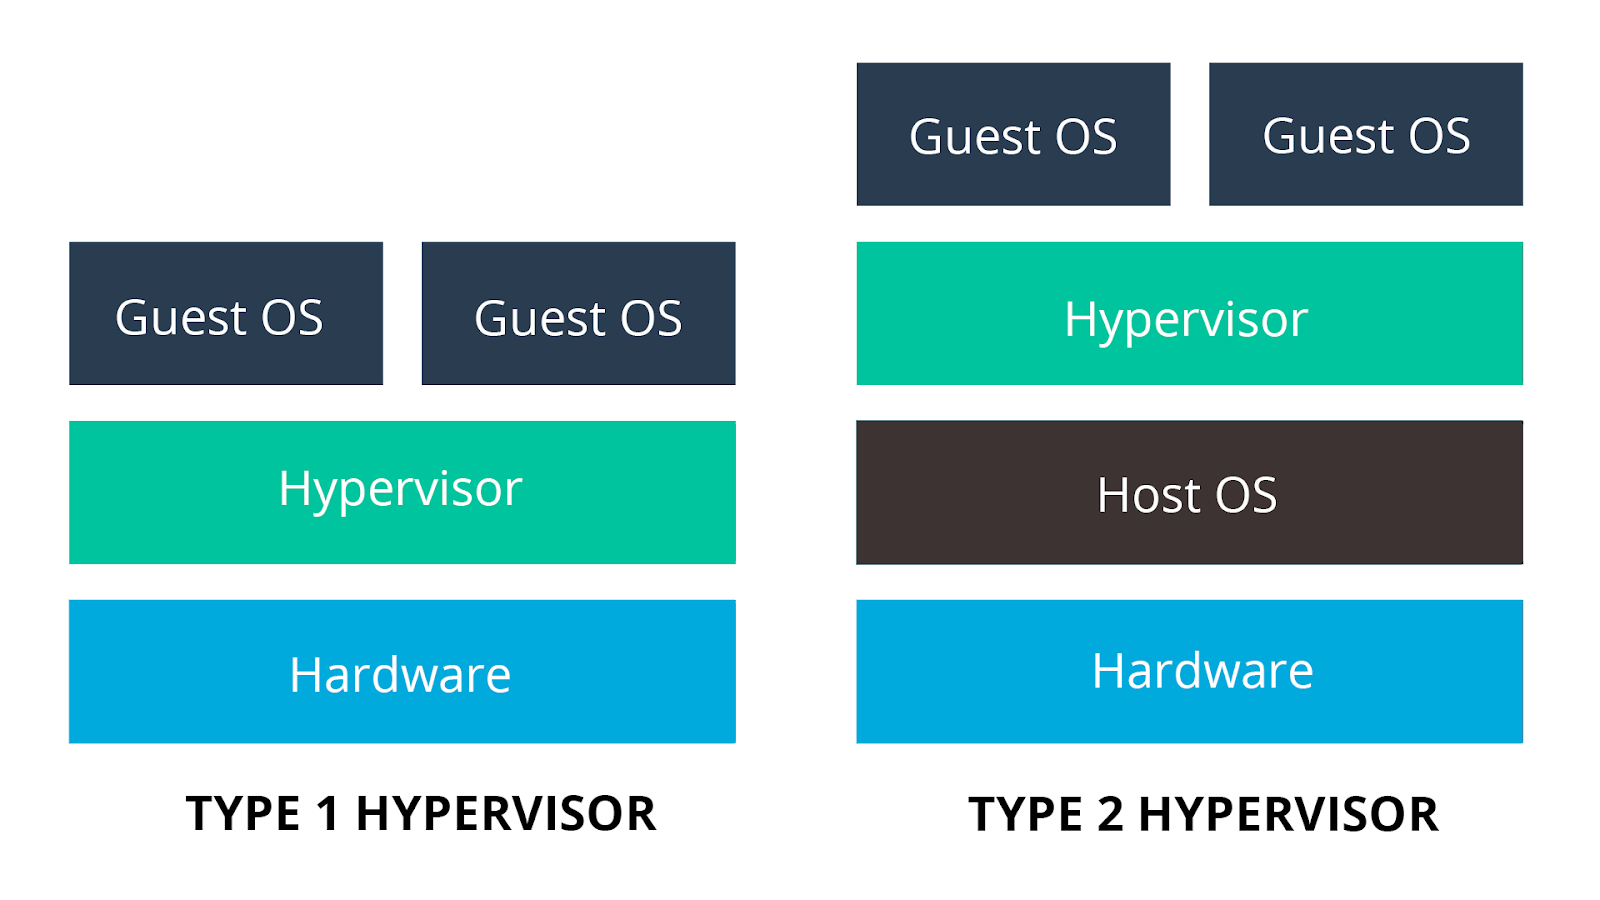
\includegraphics[width=\linewidth]{img/Hypervisor.png}
    \caption{Type 1 \& Type 2 Hypervisor \autocite{VMWare2021}}
    \label{fig:hypers}
\end{figure}

Tegenwoordig worden type 1 hypervisors in productieomgevingen het meest gebruikt, dit vanwege hun efficiënte \textit{resource} gebruik en veiligheid. Type 2 hypervisors worden meer gebruikt in testomgevingen omdat deze gemakkelijker op te zetten zijn.

Elke VM heeft zijn eigen volwaardig besturingssysteem, met gevolg dat deze veel resources gebruiken en hierbij, in vergelijking met containers, vaak trager zijn. In plaats van de onderliggende hardware te visualiseren gebruiken containers de kernel van het besturingssysteem (meestal is dit Linux) zelf, zo bevat elke individuele container enkel de applicatie en de bijhorende afhankelijkheden  \autocite{Education2020}.

\begin{figure}[ht]
    \centering
    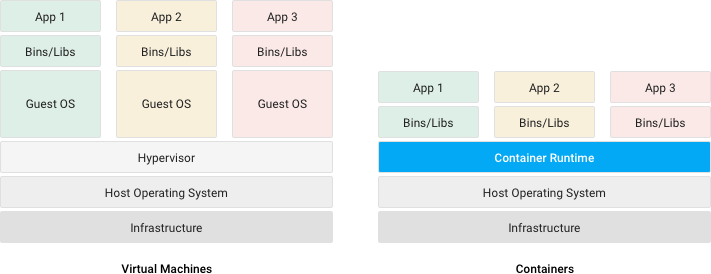
\includegraphics[width=\linewidth]{img/container-vs-vm.png}
    \caption{Container vs. virtuele machine \autocite{Google2016}}
    \label{fig:example}
\end{figure}


\subsection{Waarvoor worden containers gebruikt?}
Containers zijn zeer veelzijdig en kunnen dus in veel verschillende omstandigheden gebruikt worden. Enkele \textit{use cases} waarvoor containers zeer geschikt zijn \autocite{Docker2021}:

\begin{itemize}
  \item \underline{Microservices}: containers zijn klein en licht, waardoor ze goed passen bij microservice-architecturen waarin applicaties zijn opgebouwd uit vele, losjes gekoppelde en onafhankelijk services.
  \item \underline{Modernisering en migratie van applicaties}: een van de meest voorkomende benaderingen voor het moderniseren van applicaties begint met het containeriseren ervan, zodat ze naar de \textit{cloud} kunnen worden gemigreerd.
  \item \underline{Nieuwe ontwikkelaars snel inwerken}: door gebruik te maken van containers verloopt het opzetten van een nieuwe lokale ontwikkelingsomgeving snel en vlot, hierdoor kunnen de ontwikkelaars direct aan de slag.
\end{itemize}


\section{Docker}
\textit{Docker}\footnote{docker.com/} is een open source container platform dat sinds de \textit{release} in 2013 ongelofelijk populair is geworden. In november 2019 stond de teller van aantal \textit{pulls} op de \textit{Docker hub} op 130 miljard, in juli 2020 stond deze al op 242 miljard. Dat is bijna een verdubbeling op minder dan acht maanden tijd \autocite{Kreisa2020}. Docker-containers kunnen overal draaien, in het datacenter, bij een externe serviceprovider of in de cloud. Docker containers kunnen zowel op Linux als op Windows draaien. Containers die op Windows gebaseerd zijn kunnen echter alleen op Windows systemen draaien, maar Linux containers kunnen op zowel Linux systemen en Windows systemen draaien (met behulp van een Linux VM). Dit komt omdat containers ontworpen zijn om het besturingssysteem van de host te gebruiken \autocite{Anil2018}.


\subsection{Hoe werkt Docker?}
Docker gebruikt een \textit{Client-Server} architectuur. Deze werkt als volgt: de Docker \textit{Client} communiceert met de Docker \textit{Deamon} (een proces dat op de achtergrond draait en bepaalde (onderhouds-)taken uitvoert). Deze is verantwoordelijk voor het bouwen, runnen en verspreiden van containers \autocite{Docker2021a}.

\begin{figure}[ht]
	\centering
	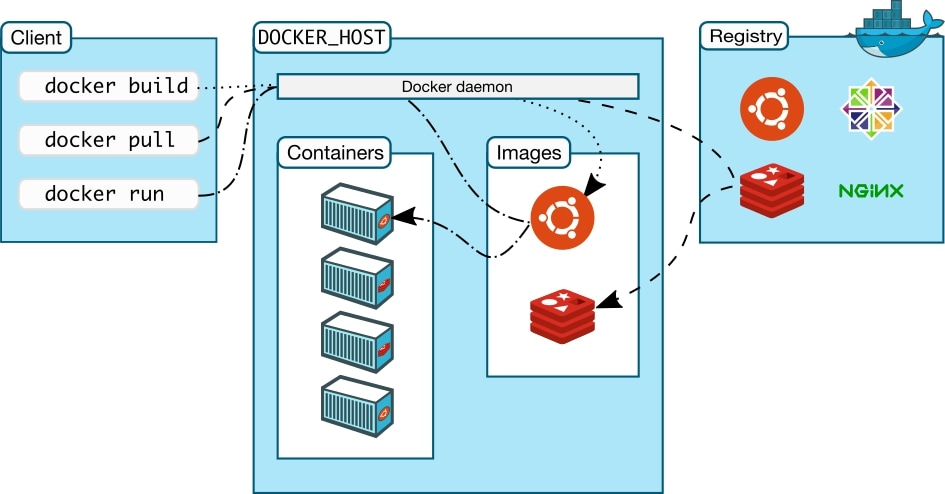
\includegraphics[width=\linewidth]{img/dockerArchitecture.jpg}
	\caption{Docker componenten \autocite{Docker2021a}}
	\label{fig:dockerArch}
\end{figure}

\subsection{Docker componenten en terminologie}

\subsubsection{Docker Deamon}De Docker Daemon (\verb|dockerd|) luistert naar Docker Application programming interface (API) verzoeken en beheert Docker objecten waaronder \textit{images}, \textit{containers}, netwerken en \textit{volumes}.

\subsubsection{Docker Client}De Docker Client is de meest gebruikte manier voor gebruikers om te communiceren met Docker. De client stuurt alle ingevoerde commando's (zoals \verb|docker pull| en \verb|docker run|) door naar de Docker Daemon die deze uitvoert.

\subsubsection{Docker registries} \label{registry}
Een \textit{Docker register} is een bibliotheek die \textit{Docker images} opslaat. Het standaard register voor Docker is de \textit{Docker Hub}\footnote{hub.docker.com/}. Als de Docker daemon geen lokale Docker image vindt gaat deze standaard in de \textit{Docker Hub} zoeken. Wanneer gebruik gemaakt wordt van de \verb|docker pull| of \verb|docker run| commando's, worden de benodigde images uit het register gehaald.

\subsubsection{Docker objecten} \label{dockerObjects}
Docker maakt gebruik van images, volumes en netwerken, al deze onderdelen worden objecten genoemd. Volgens \textcite{Docker2021a, AquaSecurity2021} zijn dit de belangrijkste objecten:

\begin{itemize}
        \item \textbf{Images}: Docker images zijn \textit{read-only} sjablonen met instructies om een Docker container op te zetten. Docker images vanuit de Docker Hub zijn typisch onmiddelijk klaar voor gebruik, zonder verdere configuratie. Verder kan je tevens bijkomende instructies toevoegen aan de \textit{base image} en deze opslaan als een nieuwe en aangepaste Docker image. Een Docker image is vaak gebaseerd op een andere image (i.e., Een nieuwe image kan gebaseerd zijn op een bestaande \textit{Ubuntu} image maar installeert en configureert daarbij een \textit{Apache} webserver). Alsook is het mogelijk om zelf een compleet nieuwe image te maken met behulp van een \textit{dockerfile}.
        \item \textbf{Containers}: een container is een uitvoerbare instantie van een image die wordt gecontroleerd via de Docker API. Een container heeft de mogelijkheid om te verbinden met andere containers, aan externe opslag of kan als basis dienen voor een nieuwe image.
        \item \textbf{Volumes}: de persistente gegevens die Docker containers kunnen gebruiken wordt opgeslagen in zogenaamde volumes. Deze volumes worden volledig gecontroleerd via de Docker API en bevinden zich buiten de container zelf. Hierdoor blijft het gewicht van de containers laag en kan de data blijven bestaan ook al wordt de container gestopt of verwijderd.
\end{itemize}

\section{Container orkestratie}
Container orkestratie helpt bij het opzetten, beheren, schalen en verbinden van een grote hoeveelheid containers. Container orkestratie helpt dus om complexe procedures te vergemakkelijken. Dit door veelvoorkomende processen en werkstromen te stroomlijnen en te optimaliseren. Een ander belangrijk onderdeel van orkestratie is het geautomatiseerd onderhoud van de applicaties die in de containers draaien \autocite{RedHat2021}.

\subsubsection{Waarvoor wordt container orkestratie gebruikt?}

Container orkestratie wordt vooral gebruikt voor het automatiseren en beheren van de configuratie en uitrol, het toewijzen van resources, de \textit{Load balancing} en het monitoren van containers.
%Container orkestratie wordt vooral gebruikt voor het automatiseren en beheren van:
%\begin{itemize}
%    \item De configuratie en uitrol van containers.
%    \item De toewijzing van resources.
%    \item De \textit{Load balancing} op basis van de belasting van het systeem.
%    \item Het monitoren van containers.
%    \item De beveiliging van interacties tussen containers.
%\end{itemize}

\subsection{Container orkestratie tools}
Om aan container orkestratie te gaan doen zijn er natuurlijk tools nodig die ons alle nodige functionaliteiten kunnen aanbieden. \textcite{DevopsCube2021} geeft een overzicht van de meest prominente orkestratie tools.

\subsubsection{Kubernetes}
Kubernetes(K8s)\footnote{kubernetes.io/} is een open source, container cluster manager en orkestratie tool. Het is gebouwd met een uitstekende resource manager voor het inzetten van containers op een efficiëntere manier. Kubernetes is voor vele organisaties de ``de facto'' container orkestratie tool geworden. Volgens \textcite{CNCF2021} zijn er meer dan 109 tools om containers te beheren, maar 89\% is gebouwd met K8s aan de basis.

\subsubsection{Openshift}
Openshift behoort tot de 89\% tools die gebouwd zijn bovenop Kubernetes. Het Openshift-project\footnote{openshift.com/} word onderhouden door RedHat\footnote{redhat.com/}. Het heeft zowel een open source versie (\textit{openshift origin}\footnote{github.com/openshift/origin}) als een enterprise versie (\textit{openshift container platform}\footnote{openshift.com/products/container-platform}).

\subsubsection{Hasicorp Nomad}
Nomad\footnote{nomadproject.io/} is een orkestratieplatform van Hashicorp\footnote{hashicorp.com/} dat containers op schaal kan ondersteunen. Op het vlak van applicatiemanagement is het zeer sterk vergelijkbaar met Kubernetes. Echter kan Nomad ook niet-containerapplicaties beheren, met gevolg dat deze zich kan distantiëren van de andere orkestratie tools. Daarnaast kan Nomad feilloos geïntegreerd worden met andere tools van Hashicorp.

\section{Kubernetes}
Hier wordt ingegaan op wat Kubernetes(K8s) doet en hoe het werkt. Daarnaast worden de verschillende technische termen die eigen zijn aan K8s uitgelegd.

Kubernetes is een \textit{open source}, container cluster manager en orkestratie tool. Het werd ontwikkeld door Google om hun container applicaties op grote schaal te kunnen orkestreren. Het project werd in 2014 \textit{open source} gemaakt, dat wil zeggen dat Google heeft besloten om het Kubernetes project samen met de \textit{community} te omwikkelen en onderhouden. Google heeft dan ook, in samenwerking met de Linux Foundation, de Cloud Native Computing Foundation(CNCF)\footnote{cncf.io/} opgericht. Zij zijn nu de \textit{maintainers} van het project en kiezen welke veranderingen er worden doorgevoerd. Hierdoor konden ook andere organisaties niet alleen gebruik maken van deze krachtige tool, maar tevens meewerken aan de ontwikkeling ervan. De term \textit{Kubernetes} is Grieks voor ``stuurman van een schip'' \autocite{Kubernetes2021}. Enkele diensten die door K8s aangeboden worden:
\begin{itemize}
    \item Automatisch load-balancing op basis van de hoeveelheid verkeer.
    \item Opslag orkestratie: Het automatisch \textit{mounten} van verschillende types opslag (lokale- of cloud opslag).
    \item Resource controle: K8s zorgt ervoor dat de beschikbare resources correct en efficiënt verdeeld worden.
    \item \textit{Self-healing}: K8s kan containers heropstarten, vervangen of stopzetten als deze niet meer voldoende correct werken.
\end{itemize}

\subsubsection{Kubernetes componenten en terminologie}
Zoals beschreven in de documentatie van \textcite{Pedersen2021, RedHat2021a} worden Kubernetes en de bijhorende componenten als volgt gedefinieerd: Kubernetes is een \textit{cluster} bestaande uit 2 grote delen namelijk het \textit{control plane} en de \textit{nodes}. Deze nodes zijn de door K8s georkestreerde containers. Elke cluster bestaat uit minstens één maar meestal meerdere nodes. De nodes worden gebruikt om \textit{pods} te hosten. Pods zijn de kleinst mogelijke eenheid in een K8s systeem. Een pod bestaat uit één of meerdere containers die opslag- en netwerk \textit{resources} delen \autocite{RedHat2021a}. In Figuur \ref{fig:K8sComponents} worden de verschillende componenten van een K8s cluster gevisualiseerd.

\begin{figure}[ht]
    \centering
    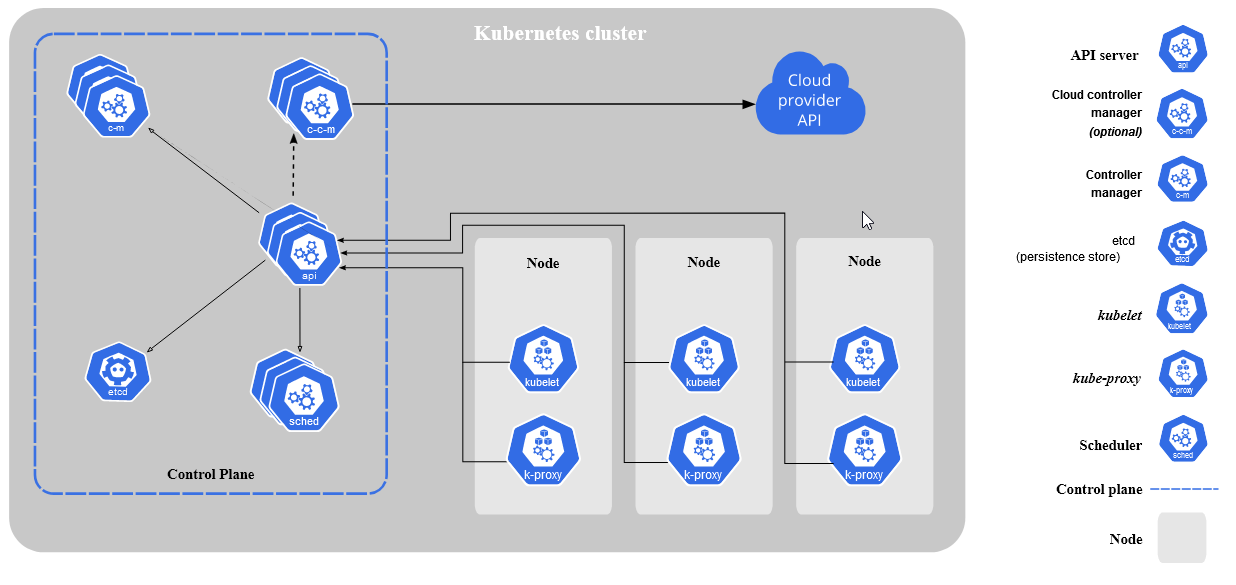
\includegraphics[width=\linewidth]{img/kubernetes-components.png}
    \caption{Kubernetes cluster componenten \autocite{Kubernetes2021}}
    \label{fig:K8sComponents}
\end{figure}

Het hart van een K8s cluster is de \textbf{\textit{Control plane}}, hierin bevinden zich alle componenten die de cluster controleren. Tevens zitten alle gegevens omtrent de staat van de cluster en de configuratie hierin verbonden. Alle componenten die deel uitmaken van de \textit{Control plane} kunnen op verschillende machines draaien. Hierbij wordt er wel aangeraden om deze binnen eenzelfde machine te houden. De verschillende onderdelen en hun plaats binnen een cluster worden hieronder besproken \autocite{Pedersen2021}.

De \textbf{\textit{kube-apiserver}} wordt gezien als de \textit{Front-end} van een Kubernetes cluster. Deze is de link tussen \textit{nodes} en \textit{pods} van de cluster en de \textit{Control plane}. Het doel van deze apiserver is om de communicatie van de nodes en de Kubernetes API te bolwerken. De apiserver is ontworpen om horizontaal te schalen als deze te zwaar belast wordt. Hierbij creëert die nieuwe instanties van zichzelf.

Alle data en informatie met betrekking tot de status van de cluster wordt opgeslagen in \textbf{\textit{etcd}}, een \textit{key-value store database}.

De \textbf{\textit{kube-scheduler}} is verantwoordelijk voor het toekennen van pods aan nodes en voor het verdelen van de resources tussen de verschillende nodes. Het toekennen van een pod aan een node gebeurd aan de hand van verschillende factoren. De mogelijke factoren zijn onder andere de benodigde resources van een pod en eventuele harware- en sofware beperkingen.

Een \textbf{\textit{kube-controller-manager}} bestaat uit verschillende \textit{controllers} die allemaal een verschillende taak op zich nemen. Enkele van deze \textit{controllers} zijn:
\begin{itemize}
    \item \textit{Node controller}: het hoofddoel van deze controller is om op te merken en correct te reageren als er nodes zouden wegvallen.
    \item \textit{Job controller}: deze zoekt naar zogenaamde \textit{job-objecten}, die eenmalige taken voorstellen, en creëert bijgevolg de nodige pods om deze taken uit te voeren.
    \item \textit{Service Account \& Token controllers}: deze creëert standaard accounts en \textit{API access tokens} voor nieuwe pods.
\end{itemize}

Als het \textit{Control plane} het hart van een K8s cluster is dan kunnen we de \textit{nodes} het lichaam noemen. Deze doen namelijk al het zware werk en worden bestuurd door de \textit{Control plane}.

Het eerste onderdeel van een node is de \textbf{\textit{kubelet}}, een kleine applicatie die op elke node aanwezig is. De \textit{kubelet} houdt de gezondheid en status van de pods, die binnen zijn node draaien, in het oog. Wanneer de \textit{Control plane} wil dat er iets gebeurd met de node zorgt de \textit{kubelet} ervoor dat deze acties correct uitgevoerd worden.

De \textbf{\textit{kube-proxy}} is een netwerk \textit{proxy} die verantwoordelijk is voor de K8s \textit{networkservices}. De \textit{kube-proxy} verzorgt netwerkcommunicatie zowel binnen- als buiten de cluster.

Het volgende component, namelijk de \textbf{\textit{Container runtime}}, werd reeds besproken in sectie \ref{containers}.

Ten slotte zijn er nog enkele extra \textit{addons} die gebruikt kunnen worden om de functionaliteit van een K8s cluster uit te breiden. Een eerste voorbeeld van een \textit{addon} is de mogelijkheid om persistent geheugen (ook wel \textit{volumes} genoemd) toe te voegen zoals uitgelegd in sectie \ref{dockerObjects}. Andere voorbeelden zijn het toevoegen van een \textbf{\textit{cluster DNS}}, \textbf{\textit{Web UI}} of \textbf{\textit{Dashboard}} en het opslaan van de log bestanden van de cluster met \textbf{\textit{cluster-level logging}}.

\clearpage
\section{Security}

Hier zal het \textit{security} aspect van containers en container orkestratie besproken worden. In dit hoofdstuk wordt er geantwoord op de onderzoeksvragen ``Wat zijn de belangrijkste beveiligingsrisico?'' en ``Welke beveiligings-tools zijn er en hoe werken ze?''.

Uit een rapport van \textcite{Tripwire2019} blijkt dat 94\% van bevraagden bezorgd zijn over de veiligheid van hun containers. Uit hetzelfde rapport blijkt ook dat 47\% zich bewust is van feit dat ze mogelijks kwetsbare containers gebruiken in hun productieomgeving. Het beveiligen van een K8s cluster is dan ook een zeer grote en complexe taak. Dit is omdat er veel verschillende onderdelen zijn die allemaal andere veiligheidsproblemen met zich mee kunnen meebrengen. Vanwege de hoeveelheid tijd en middelen die er nodig zijn voor het implementeren van goede veiligheidsmaatregelen wordt het door veel bedrijven gezien als een \textit{nice to have} in plaats van een \textit{need to have}.


\subsection{Meest voorkomende security problemen}
%Uitleg over hoe k8s security eruit ziet + wat voor exploits daarmee onmogeleijk gemaakt worden
Een van de meest voorkomende veiligheidsproblemen bij het opzetten van een K8s cluster is het fout, of zelf helemaal niet, definiëren van parameters. Dit kan er mogelijks voor zorgen dat een aanvaller kan `ontsnappen` uit een container (lees: toegang krijgen tot het host systeem). Ook het gebruik van ongecontroleerde Docker images kan ervoor zorgen dat een cluster van binnenuit gecompromitteerd kan worden.

Een ander probleem zijn de onvermijdelijke \textit{bugs} in K8s zelf. Deze is tevens wel één van de gemakkelijkste veiligheidsproblemen om op te lossen, namelijk door altijd de laatste versie van Kubernetes te installeren. Als er een \textit{bug} of kwetsbaarheid wordt ontdekt, wordt deze in de meeste gevallen binnen enkele dagen weggewerkt door het K8s security team.

\subsection{Hoe een container cluster beveiligen}
Hieronder zullen er enkele mogelijke manieren om een container cluster te beveiligen besproken worden.

\textcite{Rice2019, Lewis2019} geven enkele tips voor het veilig opzetten van een K8s cluster. Ten eerste wordt het gebruik van \textit{Role Based Access Control} (RBAC) stevig aangemoedigd. Door hiervan gebruik te maken, is het mogelijk om rollen toe te kennen aan bepaalde gebruikers. Deze rollen dicteren welke applicaties de gebruiker kan gebruiken en wat die ermee kan doen. Er zijn twee soorten rollen, namelijke \textit{Roles} en \textit{ClusterRoles}. \textit{Roles} specificeren bepaalde permissies binnen een bepaalde \textit{namespace} terwijl \textit{ClusterRoles} permissies specificeren die op de hele cluster van toepassing zijn.

Vervolgens wordt er aangeraden om nooit de administrator (ook wel \textit{root} genoemd) rechten te gebruiken, enkel als het nodig is voor de specifieke applicatie (i.e, \textit{KubeDNS}). Dit kan ervoor zorgen dat wanneer een aanvaller controle krijgt over de cluster, hij nog steeds gelimiteerd is door de restricties die aan gewone accounts worden toegekend met RBAC. Men kan tevens beter de anonieme toegang tot de API ontzeggen en vervangen door een gecontroleerde toegang met RBAC.

Via de Security Policies parameter, namelijk \verb|RunAsUser|, kan men verplichten om gebruik te maken van een normaal account. Dit wordt geïllustreerd in voorbeeld \ref{runasuser}. Een \textit{Security Policy} controleert de meer veiligheidsgevoelige aspecten van een cluster. 

Een voorbeeld van zo een policy is de \verb|seLinux| policy die, zoals zijn naam al doet vermoeden, beroep kan doen op de beveiligingsfunctionaliteiten van Security-Enhanced Linux. De \verb|volumes| policy geeft dan weer controle over de soorten volumes die gebruikt kunnen worden.

\begin{figure}[h!] \label{runasuser}
    \begin{minted}{yaml}
        apiVersion: v1
        kind: Pod
        metadata:
            name: Example
        spec:
            securityContext:
                runAsUser: 1000
    \end{minted}
\end{figure}

De communicatie tussen de pods kan gecontroleerd worden aan de hand van zogenaamde \textbf{\textit{Network policies}}. Dit zijn regels die aanduiden welke pods met elkaar kunnen communiceren en welke soort data er uitgewisseld kan worden \autocite{Venugopal2019, Bannister2021}. In voorbeeld \ref{netpolicy} wordt inkomend verkeer naar pods met label ``color: blue'' alleen toegestaan als het afkomstig is van een pod met label ``color: red'' en dit enkel op poort 80. De \textit{Network policies} kunnen handmatig worden geconfigureerd of er kan gebruik gemaakt worden van een zogenaamde \textit{Container Network Interface} (CNI). Een CNI helpt met het configureren en onderhouden van de \textit{Network policies}. In sectie \ref{Calico} wordt één van de meest prominente CNI's besproken, namelijk \textit{Project Calico}.

\begin{figure}[h] \label{netpolicy}
    \begin{minted}{yaml}
        kind: NetworkPolicy
        apiVersion: networking.k8s.io/v1
        metadata:
          name: allow-same-namespace
          namespace: default
        spec:
          podSelector:
            matchLabels:
              color: blue
          ingress:
            - from:
              - podSelector:
                  matchLabels:
                    color: red
              ports:
                - port: 80
    \end{minted}
\end{figure}

Fouten maken is menselijk, dus het is perfect mogelijk dat er tijdens het opstellen van de configuratie files enkele fouten insluipen. Daarom wordt het aangeraden om automatische \textit{configuration checks} uit te voeren zodat deze fouten vroegtijdig opgemerkt kunnen worden. Een tool die hiervoor vaak gebruikt wordt, namelijk \textbf{\textit{kube-bench}}, wordt besproken in sectie \ref{bench}.

%\textbf{\textit{uitleg over Linux security features zoals SELinux/seccomp/apparmor}}

Het spreekwoord `De ketting is maar zo sterk als zijn zwakste schakel` is ook hier van toepassing. Hoe beveiligd de cluster ook mag zijn, één onveilige container is voldoende om alle geherinvesteerde moeite teniet te doen.

Volgens \textcite{Lewis2019} zijn er verschillende manieren om ervoor te zorgen dat er enkel veilige containers gebruikt worden. De eerste is om enkel \textit{trusted base images} binnen te halen. Dit zijn containers die volledig \textit{from scratch} ontwikkeld zijn door het bedrijf, of de persoon, die container zal draaien. Dit zijn containers die volledig ontwikkeld zijn door het bedrijf dat ze in gebruik neemt. Het \textit{Base} gedeelte van de naam komt van het feit dat deze containers meestal zeer simpel zijn. Zo kan elke container applicatie gebaseerd worden op dezelfde veilige container \textit{image}.
Een extra veiligheidsmaatregel die vaak aangeraden wordt is het opzetten van een \textit{private registry}. Wat een \textit{registry} precies is werd reeds verduidelijkt in sectie \ref{registry}. Een \textit{private registry} is niets anders dan een \textit{registry} die volledig door het bedrijf wordt gecontrolleerd en enkel door hen wordt gebruikt. Zij kiezen zelf welke \textit{images} er wel of niet worden toegevoegd. Hierdoor vermijdt men dat er per ongeluk een onveilige container wordt gebouwd binnen een cluster.

Spijtig genoeg is niet iedereen die met container clusters werkt even bezorgd over de veiligheid ervan. Om het gebruik van onveilige pods te vermijden kan men een \textit{policy agent} gebruiken. Hiermee kan er automatisch gecontroleerd worden of de pods aan alle veiligheidsvoorschriften voldoen, alvorens ze ingeschakeld worden. Een voorbeeld van een \textit{policy agent} is de \textbf{\textit{Open Policy Agent}}\footnote{openpolicyagent.org/}, onwikkeld door de \textit{text Cloud Native Computing Foundation (CNCF)}.

%
%Tips:
%Gebruik ``trusted base images''
%- er wordt soms gebruik gemaakt van een private registry zodat er meer controle is op de images
%- Containers van Docker hebben een standaard Seccomp profiel dat limiteerd wat er mee kan gedaan worden (moet gespecifieerd worden in K8s)
%
%Open Policy Agent gebruiken om het opzetten van onveilige pods onmogelijk te maken adv policies.

\section{Beveiligings-tools} \label{tools}

In dit hoofdstuk zal er geantwoord worden op de onderzoeksvraag ``Welke beveiligings-tools zijn er?''

Een andere manier om een K8S cluster verder te beveiligen is om bepaalde beveiligings-tools te overwegen.
\textcite{Taylor2019} geeft een overzicht met de meest prominente tools.

\subsection{Project Calico} \label{Calico}

\textbf{\textit{Project Calico}}\footnote{projectcalico.org/} is volledig \textit{open source} en volgens \textcite{Armstrong2021} de meeste gebruikte beveiligings-tool voor K8s. Calico is niet enkel een K8s beveiligings-tool maar is tevens volledig geïntegreerd met vele andere platformen. Figuur \ref{fig:CalicaEco} geeft een overzicht van de door Calico ondersteunde platformen. Project Calico creëert een soort van \textit{microfirewall} rond elke service. De policies die ingesteld kunnen worden in Calico worden automatisch omgezet naar firewall regels. Deze worden vervolgens toegepast op elke service. Calico heeft zich onlangs aangesloten bij de CNCF, waardoor het onder deskundig toezicht staat en nog beter geïntegreerd is in het Kubernetes ecosysteem.
\begin{figure}[ht]
    \centering
    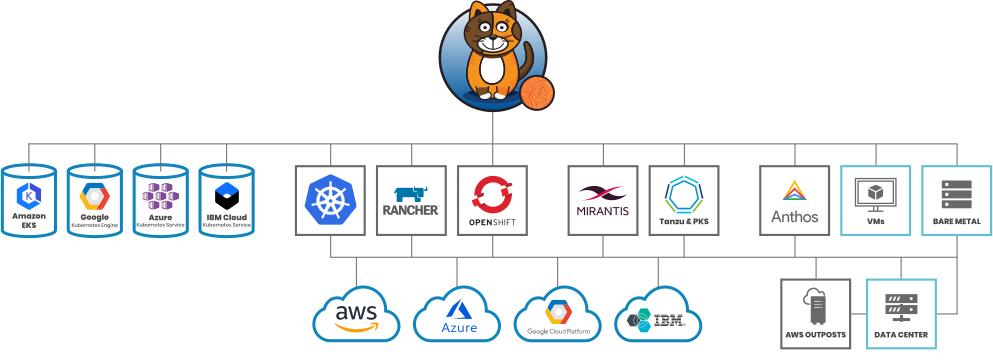
\includegraphics[width=\linewidth]{img/Calico-Ecosystem.png}
    \caption{Platformen die ondersteunt worden door Calico \autocite{Tigera2021}}
    \label{fig:CalicaEco}
\end{figure}

\subsection{Kube-Bench} \label{bench}
\textbf{\textit{Kube-Bench}}\footnote{github.com/aquasecurity/kube-bench} is een \textit{open source} applicatie geschreven in \textit{Go}\footnote{golang.org/} die controleert of K8s veilig is geïmplementeerd door middel van controles uit te voeren op de cluster. De controles zijn gebaseerd op enkele guidelines die het \textit{Center for Internet Security}\footnote{cisecurity.org/benchmark/kubernetes/} (CIS), een organisatie die richtlijnen opmaakt voor het schrijven van veilige code, heeft opgesteld. De zogenaamde \textit{CIS Kubernetes Benchmarks} worden geschreven door de Kubernetes \textit{community} en worden door de CIS gecontrolleerd en gebundeld. \textit{Kube-Bench} controleert niet alleen of er fouten in de beveiliging van een cluster zitten, het geeft ook mogelijke oplossingen. Mogelijke controles zijn het controleren van gebruikersautorisatie- en -authenticatie, de versleuteling van gegevens en kijken of de cluster het principe van \textit{least privilege} volgt (een gebruiker krijgt enkel toegang tot gegevens die hij echt nodig heeft). De testen worden gedefinieerd in een `YAML Ain't Markup Language' (YAML) bestand zodat ze gemakkelijk aangepast en uitgebreid kunnen worden \autocite{Rice2021}. De testen worden uitgevoerd op elke individuele node in de cluster waardoor het vooral geschikt is voor kleinere opstellingen.

\subsection{Kube-hunter} \label{hunter}

\textbf{\textit{Kube-hunter}}\footnote{github.com/aquasecurity/kube-hunter} is, net zoals \textit{Kube-Bench}, een open source applicatie gemaakt door \textit{Aqua Security}\footnote{aquasec.com/}. \textit{Kube-hunter} breidt de functionaliteiten van \textit{Kube-Bench} uit door penetratie testen uit te voeren op de cluster. Dit zorgt ervoor dat administrators problemen met een cluster gemakkelijk kunnen opsporen en verhelpen.

Er zijn drie verschillende manieren om \textit{kube-hunter} te gebruiken. De eerste maakt gebruik van het IP-adres van de cluster om vanop afstand de testen uit te voeren. Bij de tweede manier wordt \textit{kube-hunter} lokaal op één van de machines in de cluster geïnstalleerd om die netwerkinterfaces van die specifieke machine te testen. De derde en laatste manier om \textit{kube-hunter} te gebruiken is om het te installeren in een pod binnen de cluster. Deze manier kan aantonen wat voor potentiële schade er kan aangericht worden als één van de pods gecompromitteerd zou worden.
% !TeX spellcheck = nl_NL
%%=============================================================================
%% Methodologie
%%=============================================================================

\chapter{\IfLanguageName{dutch}{Methodologie}{Methodology}}
\label{ch:methodologie}

%% TODO: Hoe ben je te werk gegaan? Verdeel je onderzoek in grote fasen, en
%% licht in elke fase toe welke stappen je gevolgd hebt. Verantwoord waarom je
%% op deze manier te werk gegaan bent. Je moet kunnen aantonen dat je de best
%% mogelijke manier toegepast hebt om een antwoord te vinden op de
%% onderzoeksvraag.
Om het effect van zowel K8s \textit{best-practices} als K8s beveiligings-tools op een cluster te onderzoeken werd er gekozen om het onderzoek in drie scenario's onder te verdelen. Met als doel gegevens te verzamelen over enkele criteria, namelijk het resource gebruik, de stabiliteit en de opstarttijd van de cluster. Voordat we aan de scenario's kunnen beginnen, worden eerst nog alle stappen doorlopen voor het opzetten van de cluster. Nadat de cluster opgezet is zullen we beginnen met het eerste scenario, namelijk het opzetten van een basis cluster om de functionaliteit van K8s aan te tonen en om baseline gegevens te verzamelen voor het onderzoek. Deze cluster zal dienen als basis om verdere scenario's verder uit te werken. Als tweede worden er enkele ``best-practice'' gehanteerd bij het opzetten en de configuratie van de cluster, dit om te onderzoeken wat voor effect deze hebben op de cluster. Ten slotte zal er bij het opzetten en configureren van de cluster gebruik gemaakt worden van enkele K8s beveiligings-tools, dit om te testen wat deze precies doen en wat voor effect deze kunnen hebben op de criteria. 

Gedurende dit onderzoek werd er gebruik gemaakt van de volgende hardware en software:

\begin{itemize}
	\item Besturingssysteem: Pop!\_OS 20.10 x86\_64
	\item Host systeem: MSI GL62 7REX
	\item Kernel: 5.11.0-7614-generic (Linux)
	\item Cloud provider: Linode\footnote{cloud.linode.com/}
	\item Nodes: 3 X Linode 2GB (1CPU core, 2GB RAM, 50GB opslag, Debian 5.10.24-1)
\end{itemize}

\section{Opzetten van de Kubernetes cluster}
In dit hoofdstuk zal de basis cluster opgezet worden. Deze manier van werken zal ook gebruikt worden om de andere scenario's uit te voeren.

Voor het opzetten van de cluster zijn er maar drie onderdelen nodig:
\begin{itemize}
	\item Account bij een cloud provider, in dit geval Linode.
	\item Kubectl om de cluster te besturen.
	\item De Docker image om een applicatie te deployen op de cluster.
\end{itemize}

Aangezien Kubectl op zowel Linux, Windows als MacOS kan draaien, en de cluster zelf bij de cloud provider wordt gehost kunnen deze scenario's op bijna elke computer worden nagebootst. De stappen in volgende hoofdstukken worden allemaal uitgevoerd op een Linux systeem en kunnen dus verschillen op Windows of MacOS. Het is ook aangeraden om een nieuwe directory aan te maken zodat alle bestanden op éénzelfde plaats te vinden zijn.

Voor dit onderzoek zal gebruik gemaakt worden van de ingebouwde ``Linode Kubernetes Engine''(LKE). Deze installeert automatisch de correcte onderdelen op de verschillende worker nodes en creëert ook een gratis master node. Hiervoor werd gekozen omdat het volledig opzetten van een K8s cluster niet binnen de scope van dit onderzoek ligt. Door gebruik te maken van de LKE kunnen we ons dus focussen op de beveiliging van de cluster. 

\subsection{Linode Kubernetes cluster}
Hieronder worden de verschillende stappen die doorlopen zijn bij het opzetten van een Linode K8s cluster beschreven.

Voor het creëren van een cluster in Linode hebben we enkel een Linode account nodig. Het aanmaken van de cluster zelf is zeer gemakkelijk en gebeurt via cloud.linode.com > Kubernetes > Create Cluster. Vul dan de naam, regio en versie van de cluster in zoals in figuur \ref{fig:LinodeNaam}.

\begin{figure}[h]
	\centering
	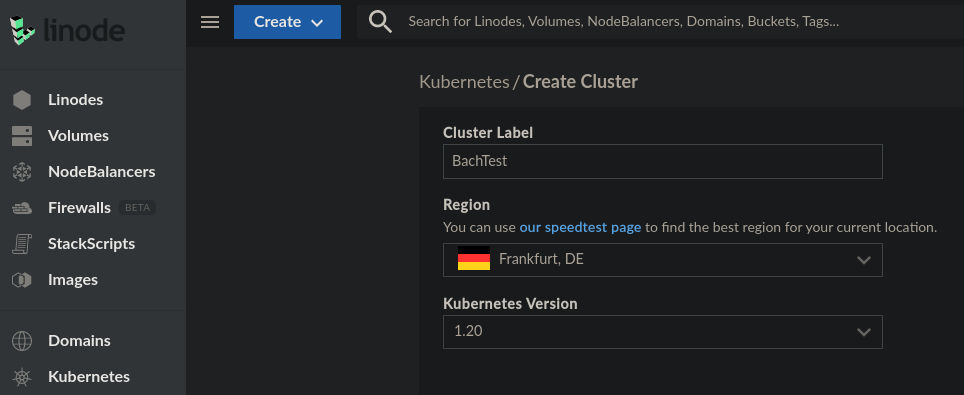
\includegraphics[width=\linewidth]{img/LinodeClusterNaam.png}
	\caption{Aanmaken Linode cluster}
	\label{fig:LinodeNaam}
\end{figure}

Vervolgens kunnen we nodes toevoegen aan de cluster. Voor dit onderzoek gaan we een kleinschalige cluster opzetten met drie worker nodes en één master node. In figuur \ref{fig:LinodeAddNodes} zijn de verschillende soorten nodes die we kunnen toevoegen opgelijst. Tijdens deze scenario's zal gebruik gemaakt worden van drie ``Linode 2GB'' nodes. Daarnaast is het ook mogelijk om nodes van verschillende groottes in dezelfde cluster toe te voegen. De master node is niet meegerekend in deze drie nodes maar word door Linode gratis aangeboden bij het opzetten van een K8s cluster.

\begin{figure}[h]
	\centering
	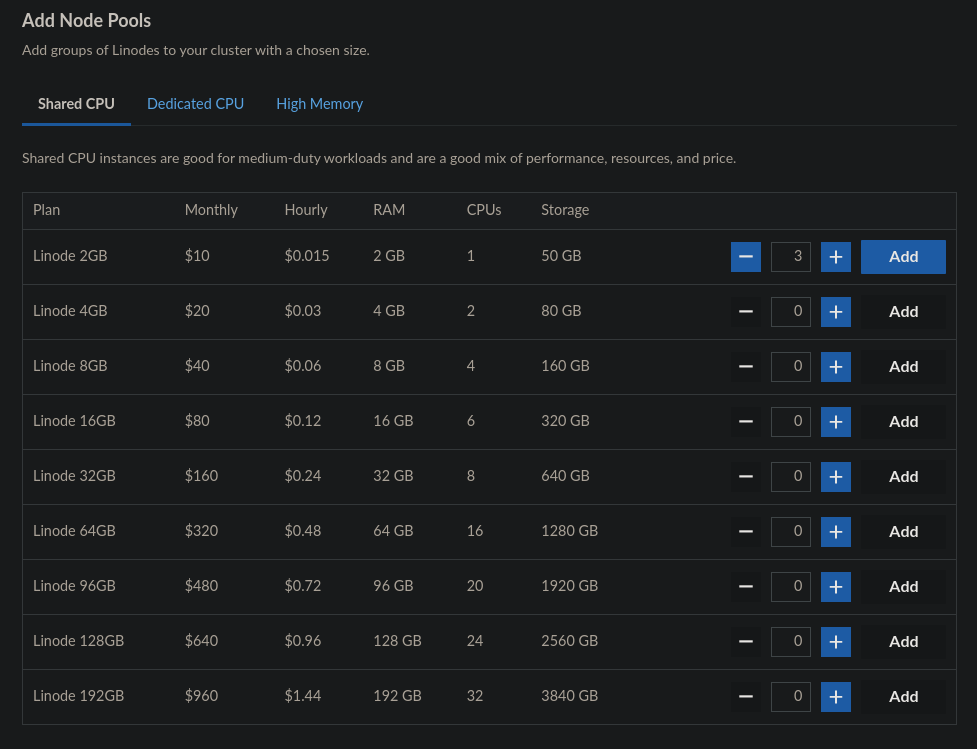
\includegraphics[width=\linewidth]{img/LinodeAddNodes.png}
	\caption{Toevoegen van nodes aan cluster}
	\label{fig:LinodeAddNodes}
\end{figure}

Als alle nodes zijn toegevoegd wordt de cluster aangemaakt. Linode zal hierbij in de achtergrond de gekozen nodes aanmaken alsook de master node klaarmaken voor gebruik. 

Eénmaal de cluster is aangemaakt en opgestart is moeten we deze nog configureren. Deze configuratie gebeurt via Kubectl in volgende stappen:

Als eerste moeten we het kubeconfig.yaml bestand downloaden van Linode. In dit bestand staan alle nodige details om Kubectl te connecteren met onze cluster. De kubeconfig van de net aangemaakte cluster is te zien in figuur \ref{kubeconfig} (enkele waarden werden ingekort om de leesbaarheid te vergroten).

\begin{figure}[h] 
	\inputminted[fontsize=\footnotesize,linenos]{yaml}{files/BachTest-kubeconfig.yaml}
	\caption{kubeconfig.yaml}
	\label{kubeconfig}
\end{figure}

Vervolgens moet het pad naar het bestand geëxporteerd worden naar de omgevingsvariabele ``KUBECONFIG'' met het volgende commando:
\begin{minted}{bash}
$ export KUBECONFIG=<pad naar file>/kubeconfig.yaml
\end{minted}

We kunnen testen of dit gelukt is door het volgende commando uit te voeren. Dit zou de drie aangemaakte nodes in onze cluster moeten teruggeven.
\begin{minted}{bash}
$ kubectl get nodes
NAME                          STATUS   ROLES    AGE    VERSION
lke25332-32960-608682818f2e   Ready    <none>   6d4h   v1.20.5
lke25332-32960-60868281f030   Ready    <none>   6d4h   v1.20.5
lke25332-32960-608682824efd   Ready    <none>   6d4h   v1.20.5
\end{minted}

Nu Kubectl in contact staat met de ``kube-apiserver'' dewelke op de master node draait, kunnen we beginnen met het configureren van onze cluster. Dit kan zowel met ``ad-hoc'' commando's als met zogenaamde deployments die werken via het \textit{principle of desired state}. Met andere woorden specificeren de deployments de verschillende  aspecten van de cluster waarbij K8s ervoor zorgt dat aan deze specificaties voldaan worden.

Een deployment is eigenlijk niets anders dan een YAML bestand waarin beschreven wordt hoe de cluster er moet gaan uitzien. Via het volgende commando wordt een deployment op een cluster gezet.
\begin{minted}{bash}
$ kubectl apply -f deployment.yaml
\end{minted}

\subsection{Resetten van cluster}
Na het uitvoeren van elk scenario zal de cluster weer worden gereset zodat het vorige scenario geen impact kan hebben op de rest van het onderzoek. Het resetten van de cluster bestaat vooral uit het verwijderen van deployments en services. Het verwijderen van een deployment wordt gedaan aan de hand van volgend commando:
\begin{minted}{bash}
$ kubectl delete deployment <Deployment naam>
\end{minted}
Het verwijderen van een service verloopt op dezelfde manier:
\begin{minted}{bash}
$ kubectl delete service <Service naam>
\end{minted}
	
\subsection{Gegevens- verzameling en verwerking} \label{ch:gegevens}
Om conclusies te kunnen trekken uit dit onderzoek hebben we gegevens nodig. Meer bepaald gegevens over de bovengenoemde criteria, namelijk het \textit{resource} gebruik, de stabiliteit en de opstarttijd van de cluster. Deze gegevens zullen gebruikt worden om de onderzoeksvraag ``Welke impact hebben \textit{best practices} en beveiligings-tools op de criteria?'' te beantwoorden. De verzameling van deze gegevens zal gebeuren via \textit{sysstat}\footnote{github.com/sysstat/sysstat}. Dit is een open source tool die ons in staat stelt om een hele hoop verschillende soorten data van ons systeem te exporteren naar bruikbare formaten (zoals JSON, CSV en XML). Deze bestanden zullen later in RStudio als bron gebruikt worden om statische modellen mee te maken. Sysstat zal op één van de nodes in de cluster worden geïnstalleerd. Dit door middel van een ssh verbinding op te zetten met één van de Nodes en dan volgend commando uit te voeren. 
\begin{minted}{bash} 
$ sudo apt-get install sysstat
\end{minted}

Vervolgens moeten we de data collectie aanzetten door in het bestand \verb|/etc/default/sysstat| de variabele \verb|ENABLED| van\textit{''false''} naar \textit{''true''} om te zetten. Vanaf nu zal een van de meegeleverde tools, namelijk sar, elke 10 minuten een nieuwe entry maken in het bestand \verb|/var/log/sysstat/sa<dag van de maand>|. We kunnen deze bestanden uitlezen met behulp van het \verb|sar| commando. Om het CPU gebruik van het systeem om te zetten naar een csv bestand, om het later in RStudio te verwerken, kunnen we het volgende commando gebruiken. In figuur \ref{fig:CPUDataPreview} is het net gecreëerde csv bestand te zien.

\begin{minted}{bash} 
$ sar -f /var/log/sysstat/sa08 >> /root/CpuGebruikDag8.csv
\end{minted}

\begin{figure}[h]
	\centering
	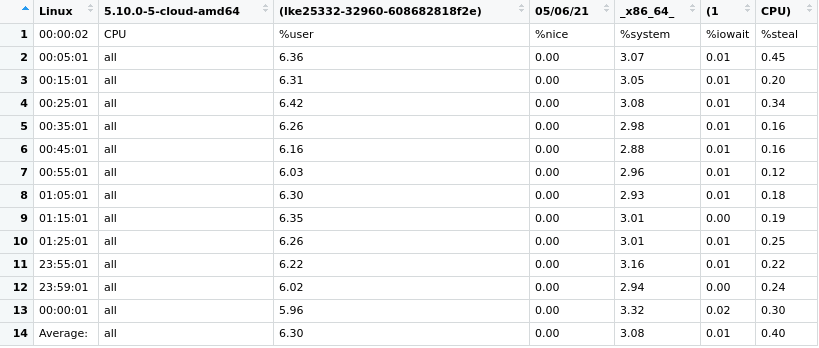
\includegraphics[width=\linewidth]{img/CPUDataPreview.png}
	\caption{Klein deel van het gebruikte csv bestand}
	\label{fig:CPUDataPreview}
\end{figure}

Vervolgens kunnen we door andere \textit{flags} mee te geven aan het sar commando verschillende soorten data uit de logbestanden halen. Het RAM gebruik kan bijvoorbeeld met volgend commando in een csv bestand worden opgeslagen:

\begin{minted}{bash} 
$ sar -f /var/log/sysstat/sa08 -r >> /root/RAMGebruikDag8.csv
\end{minted}

Als laatste moeten de gegevens lokaal op de computer beschikbaar zijn. Dit wordt gedaan door een SFTP verbinding te maken met de node waar sysstat op geïnstalleerd is en de volgende commando's uit te voeren:

\begin{minted}{bash} 
$ sftp root@172.105.86.96
root@172.105.86.96 s password:
Connected to 172.105.86.96.
sftp> lcd /home/nick/Desktop
sftp> get CpuGebruikDag8.csv
Fetching /root/CpuGebruikDag8.csv to CpuGebruikDag8.csv
\end{minted}

Nu alle nodige gegevens zijn verzamelt kan er begonnen worden aan het verwerken van deze gegevens. Dit wordt gedaan door gebruik te maken van R en Rstudio. 

Het eerste criteria is het vergelijken van het gemiddeld resource gebruik van zowel de CPU als het RAM geheugen. Voor het CPU gebruik kan dit simpelweg door de laatste rij van het csv bestand af te lezen. Het gemiddeld gebruik van het RAM geheugen wordt niet automatisch gegenereerd door sar en moet nog berekent worden. De R code om dit te doen wordt beschreven in figuur \ref{RAMAVG}.

\begin{figure}[h] 
	\inputminted[fontsize=\footnotesize,linenos]{R}{files/dataRAMAVG.R}
	\caption{R code om boxplot van CPU gegevens te bekomen}
	\label{RAMAVG}
\end{figure}
%

Het tweede criteria is de stabiliteit van het systeem. Dit zal onderzocht worden door een Boxplot te maken op basis van de verzamelde gegevens om de hoeveelheid outliers visueel voor te stellen. De R code om dit te doen voor het CPU gebruik staat in figuur \ref{CPUBox}. In dit R script wordt het csv bestand eerst ingelezen zonder de eerste rij omdat deze niet nuttig is voor het verdere onderzoek. Vervolgens houden we enkel de achtste kolom over omdat hier de hoeveelheid ongebruikte CPU kracht staat. Deze wordt dan afgetrokken van honderd om zo tot de gebruikte hoeveelheid CPU te komen. Als laatste wordt de naam van kolom veranderd zodat het gemakkelijker is om deze te gebruiken bij het maken van de boxplot. De laatste lijnen van het script zijn verantwoordelijk voor het creëren en opmaken van de boxplot.

\begin{figure}[h] 
	\inputminted[fontsize=\footnotesize,linenos]{R}{files/dataCpuBox.R}
	\caption{R code om boxplot van CPU gegevens te bekomen}
	\label{CPUBox}
\end{figure}
%
%\begin{figure}[h]
%	\centering
%	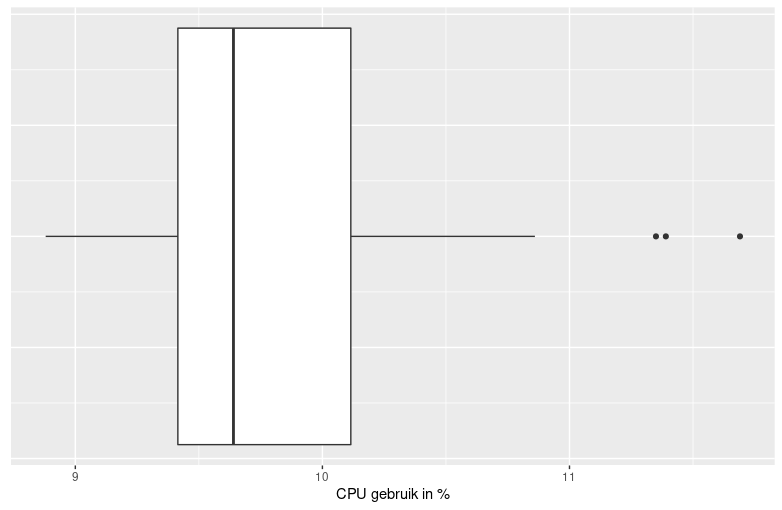
\includegraphics[width=\linewidth]{img/CPUBoxEx.png}
%	\caption{Voorbeeld boxplot CPU data}
%	\label{fig:CPUBoxEx}
%\end{figure}

Voor de gegevens van het RAM gebruik wordt op dezelfde manier te werk gegaan. De R code om de gegevens met betrekking tot het RAM geheugen wordt beschreven in figuur \ref{RAMBox}.
\begin{figure}[h] 
	\inputminted[fontsize=\footnotesize,linenos]{R}{files/dataRAMBox.R}
	\caption{R code om boxplot van CPU gegevens te bekomen}
	\label{RAMBox}
\end{figure}

Om ervoor te zorgen dat we de stabiliteit van de verschillende scenario's  met elkaar kunnen vergelijken is het ook nodig om te weten hoeveel \textit{outliers} er precies aanwezig zijn. Dit is niet altijd zo gemakkelijk te tellen als deze kort bij elkaar liggen. De \textit{outliers} kunnen allemaal opgelijst worden met het volgend commando:
\begin{minted}{bash} 
> boxplot(ram)$out
[1] 60.90 60.96 61.01 61.07 61.06 61.16 61.20 61.21 61.31 61.29 61.35
[12] 61.49 61.44 61.49 61.55 61.59 61.68 61.72 61.78 61.76 61.80 61.84
[23] 61.95 61.95 61.99 62.04 62.13 62.17 62.30 62.43 62.39 62.43 62.47
\end{minted}

Als derde criteria zal er gekeken worden naar het algemene resource gebruik van de cluster. Deze zal voorgesteld worden als een lijngrafiek waarin het resource gebruik van zowel de CPU als het RAM geheugen worden voorgesteld ten opzichte van de tijd. Het R script om dit te bekomen staat in figuur \ref{CPUGraph}. 

\begin{figure}[h] 
	\inputminted[fontsize=\footnotesize,linenos]{R}{files/dataCpuGraph.R}
	\caption{R code om grafiek van CPU gegevens te bekomen}
	\label{CPUGraph}
\end{figure}

%\begin{figure}[h]
%	\centering
%	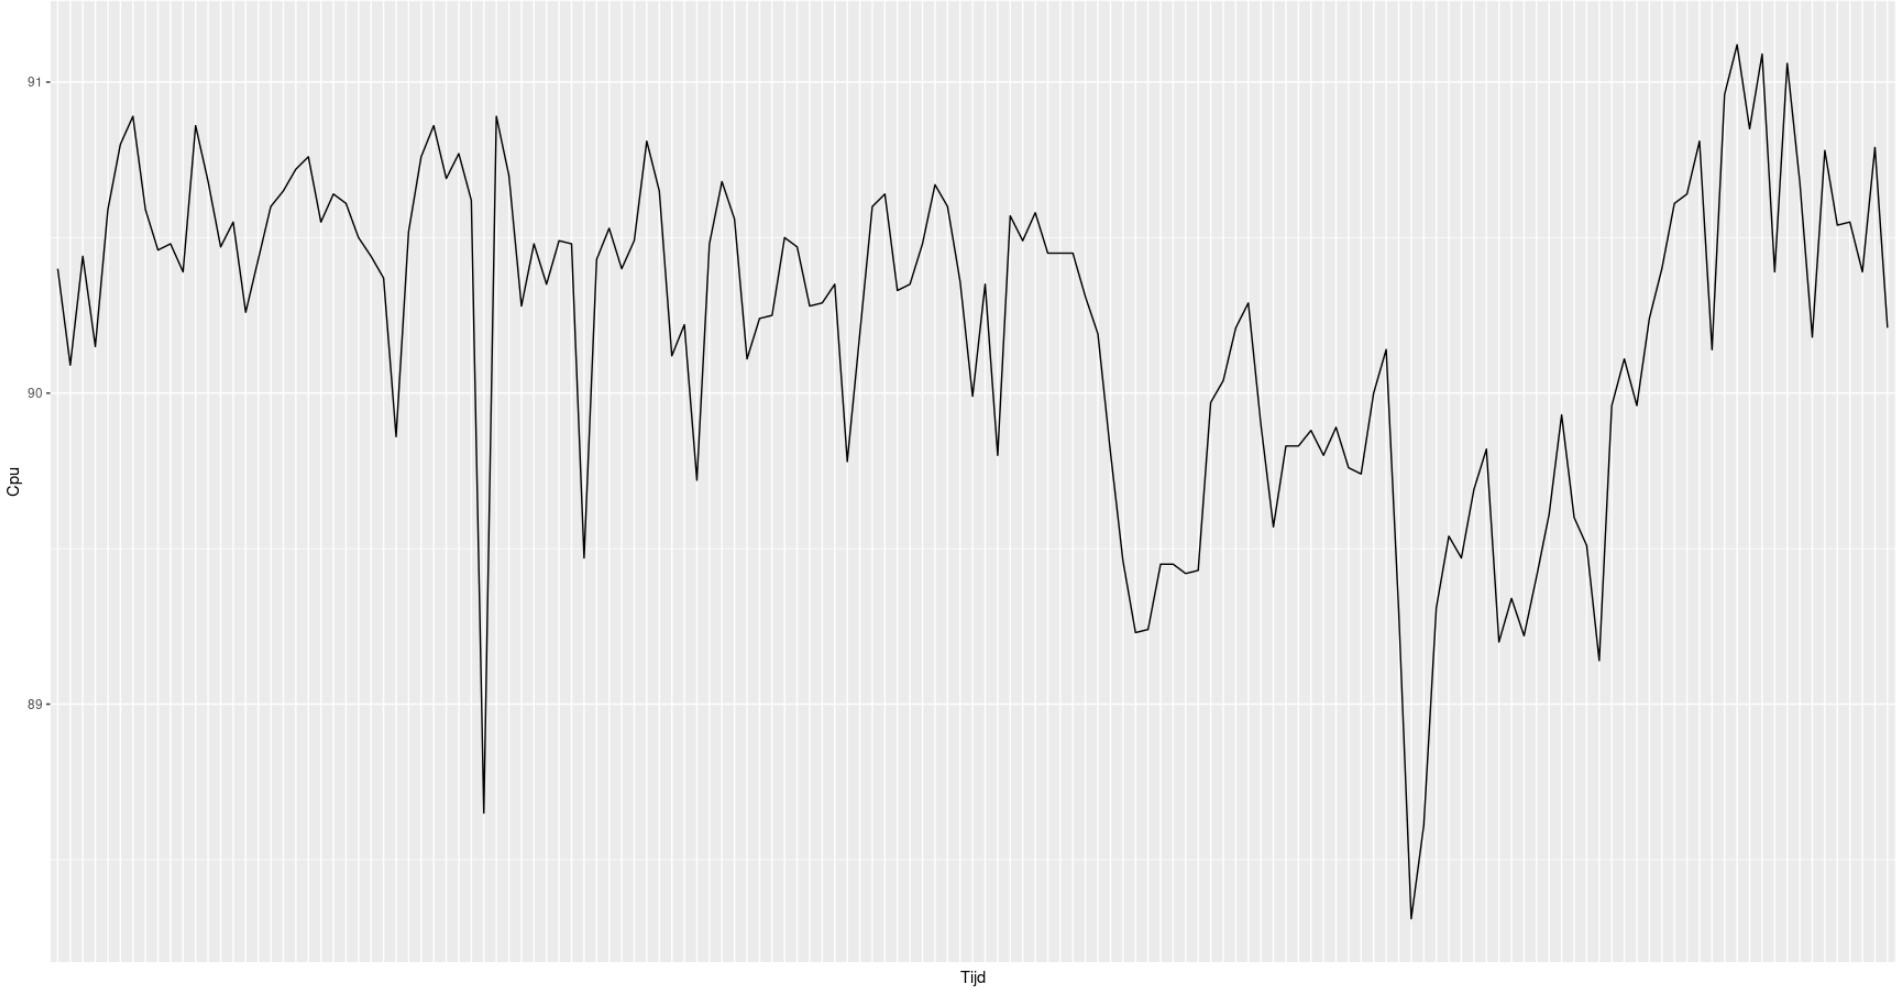
\includegraphics[width=\linewidth]{img/CPUGraphEx.png}
%	\caption{Voorbeeld grafiek CPU data}
%	\label{fig:CPUgraphEx}
%\end{figure}
Als laatste criteria zal de tijd die de node nodig heeft om op te starten vergeleken worden. Dit kan simpelweg door het volgende commando uit te voeren op de node:
\begin{minted}{bash} 
$ systemd-analyze
\end{minted}

\clearpage
\section{Scenario 1: Cluster opstelling zonder oog voor security}
%\begin{itemize}
%	\item Basic deployment van een statische website uitleggen aan de hand van commando's, screenshots en config files. 
%	\item deployment YAML tonen en deels uitleggen
%	\item Service YAML tonen en deels uitleggen
%	\item Nodige gegevens uit de cluster halen met sysstat
%	\item Verzamelde gegevens verwerken met RStudio en grafieken/statistieken tonen en uitleggen.
%\end{itemize}

%Het eerste scenario bestaat eruit om een simpele cluster op te zetten zonder specifiek oog te hebben voor de beveiliging. De deployment die zal gebruikt worden wordt in figuur \ref{basicDeploy} weergegeven. Hierin wordt een simpele demo website opgezet door gebruik te maken van de image \verb|thenetworkchuck/nccoffee:pourover|. Het aantal pods dat wordt gecreëerd wordt bepaald door de waarde van de \verb| replicas| variabele, in dit geval worden er 3 pods gecreëerd. Er wordt aangeraden om in een productieomgeving het aantal pods en nodes ongeveer gelijk te houden. De variabele \verb|imagePullPolicy: Always| zorgt ervoor dat de Docker image telkens moet worden gedownload van de registry, ook al is deze locaal aanwezig. 
Het eerste scenario bestaat eruit om een simpele cluster op te zetten zonder specifiek oog te hebben voor de beveiliging. De deployment die zal gebruikt worden wordt in figuur \ref{basicDeploy} weergegeven. Enkele van de variabelen worden hieronder uitgelegd: 
\begin{itemize}
	\item \verb|image: thenetworkchuck/nccoffee:pourover|: dit is de Docker image met de statische demo site.
	\item \verb|replicas:3|: het aantal pods die moeten worden gecreëerd wordt door deze variabele ingesteld. In dit geval zijn dat er drie.
	\item \verb|imagePullPolicy: Always|: deze variabele zorgt er in dit scenario voor dat de Docker image steeds word gedownload uit de \textit{registry} als de \textit{deployment} wordt gebruikt.
	\item \verb|containerPort: 80|: dit zorgt ervoor dat de site via poort 80 beschikbaar zal zijn.
\end{itemize}

\begin{figure}[h] 
	\centering
	\inputminted[fontsize=\footnotesize,linenos]{yaml}{files/deployment.yaml}
	\caption{deployment.yaml}
	\label{basicDeploy}
\end{figure}

Als het \textit{deployment} YAML bestand klaar is, kan deze met volgend commando op de cluster gezet worden:
\begin{minted}{bash} 
$ kubectl apply -f deployment.yaml
\end{minted}
Het opzetten van de pods kan gevolgd worden met het volgende commando. In figuur \ref{fig:getPodsDeployment1} is te zien hoe de pods één voor één klaargemaakt worden.
\begin{minted}{bash} 
$ kubectl get pods
\end{minted}

\begin{figure}[h]
	\centering
	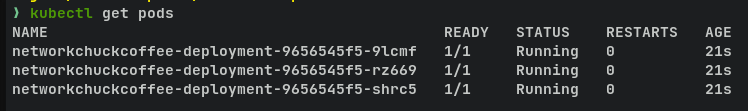
\includegraphics[width=\linewidth]{img/kubectlGetPodsDeployment1.png}
	\caption{Pods worden klaargemaakt}
	\label{fig:getPodsDeployment1}
\end{figure}

Als we nu de \textit{deployment} willen aanpassen zonder de cluster volledig af te breken kunnen we het commando 
\begin{minted}{bash} 
$ kubectl edit deployments networkchuckcoffee-deployment
\end{minted}
gebruiken. In figuur \ref{editDeploy1} is de output van dit commando te zien. Als we in dit bestand bijvoorbeeld de \verb|replicas| variabele zouden aanpassen en het bestand opslaan, zal K8s merken dat er iets is veranderd. Omdat er gebruik wordt gemaakt van het ``Principle of desired state'' zal er automatisch aan de nieuwe specificaties worden voldaan. Om dit aan te tonen zal de variabele veranderd worden van drie naar vijf.

%\begin{figure}[ht]
%	\centering
%	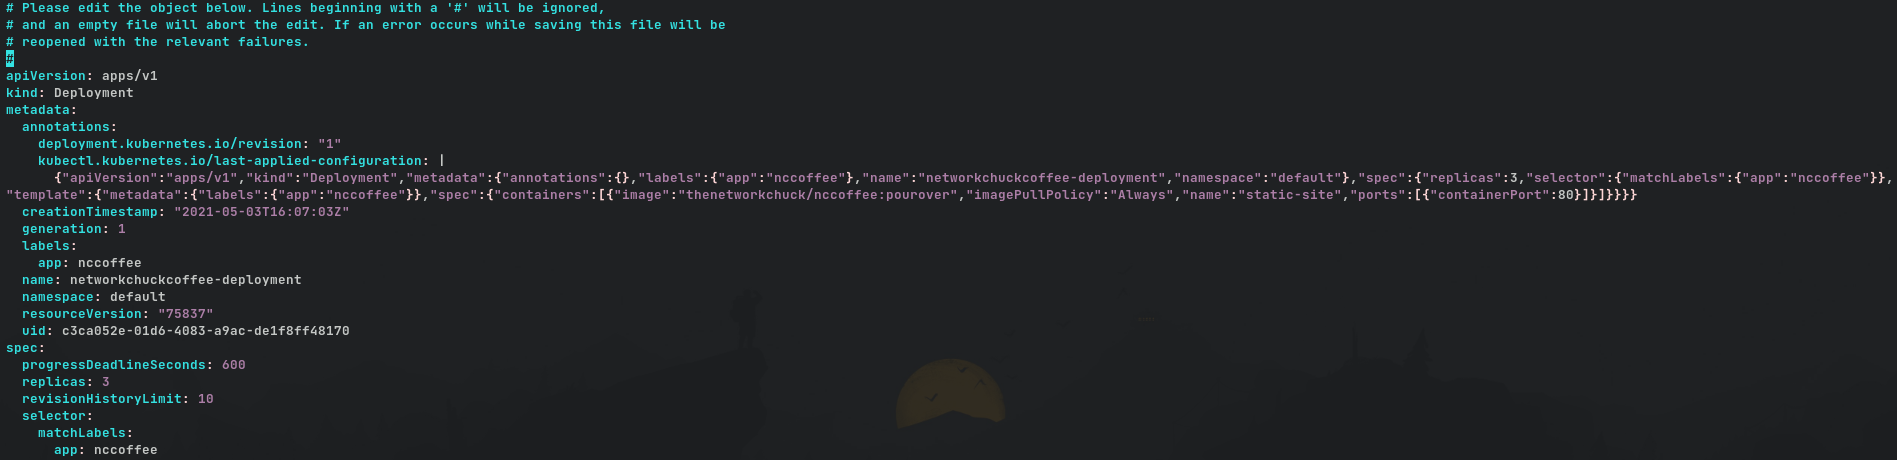
\includegraphics[width=\linewidth]{img/editDeployment1.png}
%	\caption{Output ``kubectl edit deployments'' commando}
%	\label{fig:editDeployment1}
%\end{figure}

\begin{figure}[h] 
	\inputminted[fontsize=\footnotesize,linenos]{yaml}{files/editDeployment.yaml}
	\caption{Output ``kubectl edit deployment'' commando}
	\label{editDeploy1}
\end{figure}

Als we het aantal replicas verhoogd hebben van drie naar 5 en het \verb|kubectl get pods| commando uitvoeren krijgen we, zoals in figuur \ref{fig:kubectlGetPodsEditDeploy1} te zien, dat er twee extra pods worden bijgemaakt. Deze pods worden via de \textit{scheduler} op de master node verdeeld over de drie nodes in onze cluster.
\begin{figure}[h]
	\centering
	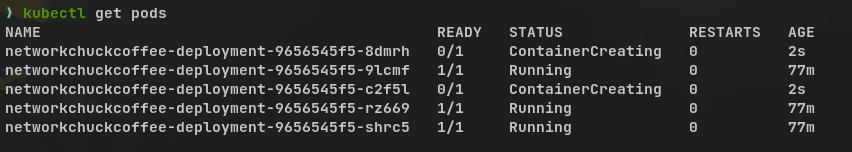
\includegraphics[width=\linewidth]{img/kubectlGetPodsEditDeploy1.png}
	\caption{Extra pods worden klaargemaakt}
	\label{fig:kubectlGetPodsEditDeploy1}
\end{figure}

Nu we klaar zijn met het opzetten van de \textit{deployment} is het mogelijk om de cluster bloot te stellen aan het internet. Momenteel is het nog niet mogelijk om de site van buiten de cluster te bekijken. Dit komt omdat er nog geen \textit{service} draait die de cluster openzet naar het internet. De service die hier zal opgezet worden zal een \textit{loadbalancer} creëren op Linode die automatisch al het verkeer verdeeld over alle pods in de cluster. Het YAML bestand om de service aan te maken is te zien in figuur \ref{service1}. De code \verb|selector:app: nccoffee| zorgt ervoor dat de \textit{loadbalancer} het verkeer tussen alle pods waar de applicatie ``nccoffee'' op draait verdeelt. Wanneer er pods bijkomen of verdwijnen zal de loadbalancer zich automatisch aanpassen. 

\begin{figure}[h] 
	\inputminted[fontsize=\footnotesize,linenos]{yaml}{files/testservice.yaml}
	\caption{service.yaml}
	\label{service1}
\end{figure}

Het volgend commando kan gebruikt worden om het publieke IP-adres van de \textit{loadbalancer} te vinden:
\begin{minted}{bash} 
$ kubectl get services
\end{minted}

Er is ook een manier om een meer gedetailleerde beschrijving van de service te krijgen. Namelijk door middel van het volgend commando:
\begin{minted}{bash} 
$ kubectl describe services coffee-service 
\end{minted}

In figuur \ref{fig:kubectlDescriveService1} is de output van dit commando en alle informatie over de \textit{loadbalancer service} te zien. De IP-adressen die worden getoond bij \verb|Endpoints| zijn de IP-adressen van alle achterliggende pods waar de ``nccoffee'' applicatie op draait. Als er nu naar het publieke IP-adres van de loadbalancer wordt gesurft is de demo website te zien zoals in figuur \ref{fig:demoSite1}.

\begin{figure}[h]
	\centering
	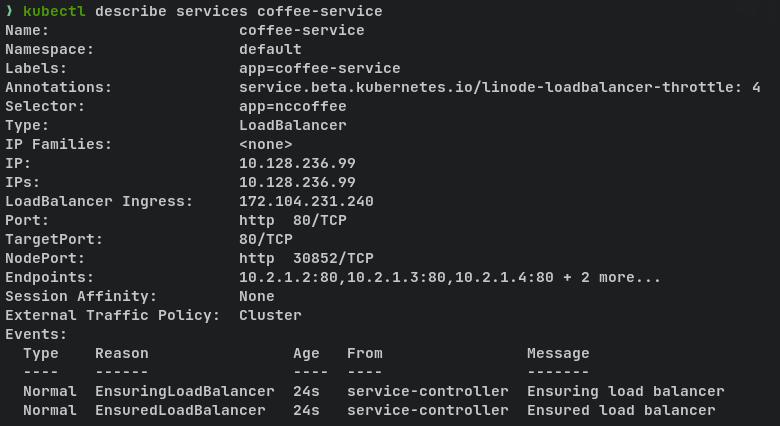
\includegraphics[width=\linewidth]{img/kubectlDescriveService1.png}
	\caption{Informatie over de loadbalancer service.}
	\label{fig:kubectlDescriveService1}
\end{figure}

\begin{figure}[h]
	\centering
	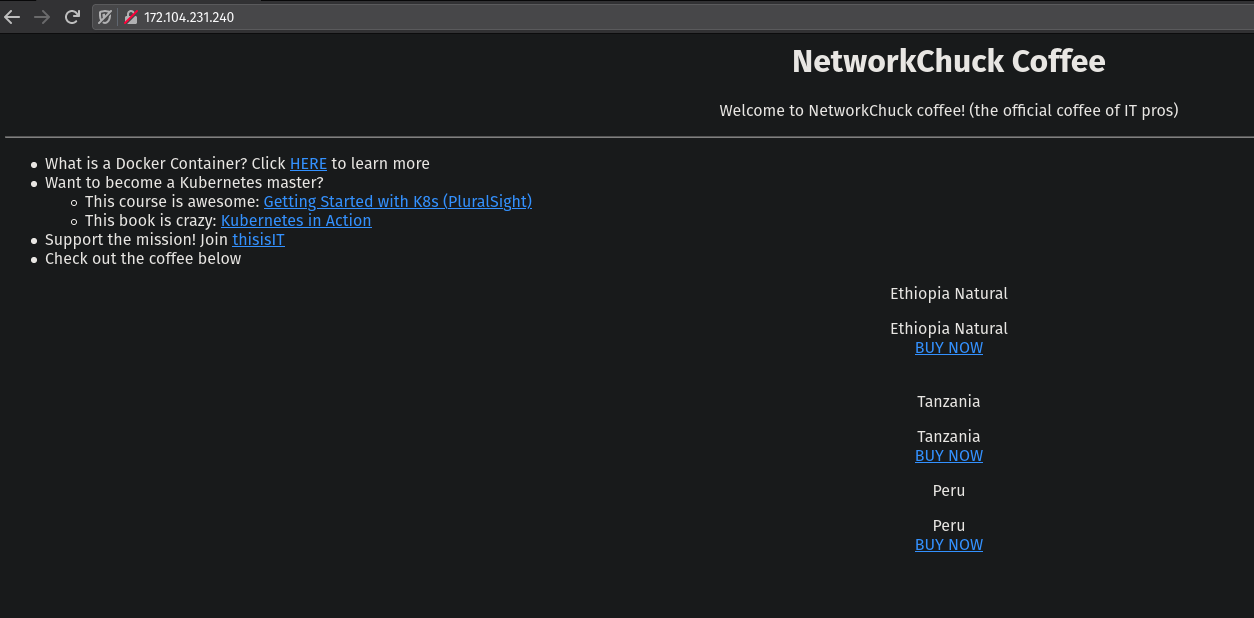
\includegraphics[width=\linewidth]{img/demoSite1.png}
	\caption{De demo website is nu zichtbaar vanop het internet.}
	\label{fig:demoSite1}
\end{figure}

\clearpage
\section{Scenario 2: Cluster opstelling met gebruik van best practices}
Het tweede scenario bestaat eruit om een simpele cluster op te zetten en gebruik te maken van enkele \textit{security best practices}. \textit{Best-practices} zoals het gebruik maken van een \textit{trusted base image} en een \textit{privite registry} zullen niet gebruikt worden omdat deze vooral dienen om de ontwikkeling van een container applicatie te beveiligen. \textit{Pod Security Policies} en \textit{RBAC} zullen wel toegepast worden op de cluster. 

Als eerste zullen er enkele Security Policies geconfigureerd worden. Het ``PodSecurityPolicy.YAML'' bestand is te zien in figuur \ref{securePol}, enkele van de variabelen worden hieronder uitgelegd: 

%https://kubernetes.io/docs/concepts/policy/pod-security-policy/

\textbf{seccomp.security.alpha.kubernetes.io/defaultProfileName:'runtime/default'}: op Linode worden nodes automatisch vooraf geïnstalleerd en geconfigureerd met AppArmor (gelijkaardig aan SELinux). Deze variabele zorgt ervoor dat de standaard \textit{container runtime} profiel wordt gebruikt. Nog een mogelijke optie is \textit{Docker runtime engine} (in dit geval werd deze al standaard ingesteld).

\textbf{privileged: false} beslist of er geprivilegieerde pods aangemaakt kunnen worden. Dit staat standaard op ``false'' en moet enkel op ``true'' gezet worden wanneer een pod andere onderdelen van de host nodig heeft om te werken. 

\textbf{allowPrivilegeEscalation: false}: dit zorgt ervoor dat de user ID niet kan veranderd worden. Een ``child-process'' kan hierdoor dus ook nooit meer privileges krijgen dan de ``Parent-process''. Door deze boolean op ``false'' te zetten wordt het moeilijker voor een aanvaller om aan ``privilege escalation'' te doen.

\textbf{hostNetwork: false}: deze variabele geeft een pod de mogelijkheid om het netwerk van de host te gebruiken. Zo kan deze ook applicaties, die via de \textit{localhost} werken, zien en deze aanpassen. Het wordt hier op ``false'' gezet omdat deze functie niet nodig is.

\textbf{runAsUser: MustRunAsNonRoot}: hier wordt de user ID gecontroleerd waarmee de pods worden aangemaakt. De waarde ``MustRunAsNonRoot'' zorgt ervoor dat de containers niet door de root gebruiker kunnen worden aangemaakt. Dit wordt vooral gebruikt om te voorkomen dat iemand die (ongewenst) root privileges heeft verkregen nieuwe (onveilige) containers kan creëren.

\textbf{SupplementalGroups: 'MustRunAs'} verplicht hier het gebruik van een ``non-root'' groep bij het aanmaken van nieuwe pods. 

\textbf{ReadOnlyRootFilesystem: false} laat het aanmaken van containers met een aanpasbare ``root filesystem'' toe. Door deze variabele op ``true'' te zetten zou elke nieuwe container aangemaakt worden met een ``Read-only root filesystem''.

\begin{figure}[h] 
	\centering
	\inputminted[fontsize=\footnotesize,linenos]{yaml}{files/securePol.yaml}
	\caption{securePol.yaml}
	\label{securePol}
\end{figure}

Nadat de PodSecurityPolicy is opgesteld kan deze met volgend commando op de cluster toegepast worden:
\begin{minted}{bash} 
$ kubectl create -f securePol.yaml
\end{minted}

De PodSecurityPolicies die op de cluster actief zijn kunnen met volgend commando opgevraagd worden:

\begin{minted}{bash} 
$ kubectl get psp
NAME        PRIV   SELINUX    RUNASUSER         SUPGROUP  READONLYROOTFS   
restricted  false  RunAsAny   MustRunAsNonRoot  MustRunAs false          
\end{minted}


Vervolgens zal er een zeer simpele testimplementatie van RBAC opgesteld worden. In figuur \ref{roleDeploy} is een kleine \textit{role} gedefinieerd, deze is verantwoordelijk voor het beheren van specifieke persmissies. In de \textit{role} die hier wordt gebruikt zorgt de \verb|resources:| variabele ervoor dat de permissies voor zowel de \textit{deployments} als de pods worden meegegeven. De \verb|verbs: ["*"]| optie is verantwoordelijk voor het aanduiden van de verschillende acties die ondernomen kunnen worden (in dit geval worden alle acties toegestaan). Het YAML bestand om de \textit{role binding} te implementeren is te zien in figuur \ref{roleBindDeploy}. Een \textit{RoleBinding} koppelt een bepaalde \textit{role} aan één of meerdere gebruikers. 
\begin{figure}[h] 
	\centering
	\inputminted[fontsize=\footnotesize,linenos]{yaml}{files/role-deployment.yaml}
	\caption{role-deployment.yaml}
	\label{roleDeploy}
\end{figure}

\begin{figure}[h] 
	\centering
	\inputminted[fontsize=\footnotesize,linenos]{yaml}{files/rolebinding-deployment.yaml}
	\caption{rolebinding-deployement.yaml}
	\label{roleBindDeploy}
\end{figure}

De \textit{role} en \textit{rolebinding} kunnen op de cluster worden aangemaakt door gebruik te maken van de \verb|create| commando's in figuur \ref{createRoles}.

\begin{figure}[h] 
	\centering
\begin{minted}{bash} 
$ kubectl create -f role-deployement.yaml
role.rbac.authorization.k8s.io/deployment-manager created
$ kukubectl create -f rolebinding-deployment.yaml
rolebinding.rbac.authorization.k8s.io/deployment-manager-binding created
\end{minted}
	\caption{Commando's voor het aanmaken van \textit{Roles} en \textit{Role Bindings}}
	\label{createRoles}
\end{figure}

\clearpage
\section{Scenario 3: Cluster opstelling met beveiligings-tools}
In dit laatste scenario zal er gewerkt worden met de beveiligings-tools die besproken zijn in sectie \ref{tools}. Project Calico zal niet worden getest aangezien deze automatisch wordt gebruikt in de LKE en het niet mogelijk is om deze te configureren. Kube-bench en Kube-hunter zullen wel uitgetest worden. De installatie en gebruik van deze tools wordt hieronder gedemonstreerd.

Als eerste is Kube-bench aan de beurt. Zoals beschreven in sectie \ref{bench} zal Kube-bench de node gaan testen tegen de \textit{CIS kubernetes Benchmarks} en een overzicht geven van de conformiteit ervan. Om Kube-bench te installeren is het nodig om een SSH verbinding op te zetten met een node in de cluster. Wanneer de verbinding gemaakt is kunnen de volgende commando's uitgevoerd worden om de installatie te voltooien.

\begin{minted}{bash} 
$ curl -L https://github.com/aquasecurity/kube-bench/releases/download/
v0.3.1/kube-bench_0.3.1_linux_amd64.deb
-o kube-bench_0.3.1_linux_amd64.deb
$ sudo apt install ./kube-bench_0.3.1_linux_amd64.deb -f
\end{minted}

Kube-bench kan nu gebruikt worden om de conformiteit van de cluster te controleren. Dit kan op verschillende manieren door enkele \textit{flags} mee te geven aan de applicatie. Configuratie van kube-bench kan op de volgende manieren gebeuren:
\begin{itemize}
	\item \verb|$ kube-bench --benchmark cis-1.5| zal er voor zorgen dat de node wordt gecontroleerd op basis van de \textit{CIS benchmark} versie 1.5. Andere opties zijn: cis-1.6, gke-1.0(Google K8s engine), eks-1.0(Elastic K8s engine) en ack-1.0. GKE, EKS en ACK staan respectievelijk voor Google Kubernetes Engine, Elastic Kubernetes Engine en AWS Controllers for Kubernetes. Deze drie opties zorgen ervoor dat er checks worden uitgevoerd die specifiek voor die platformen zijn geschreven.
	\item \verb|$ kube-bench run --targets master,node|: door dit commando uit te voeren worden enkel de test met betrekking tot de \textit{master}- en \textit{worker nodes} uitgevoerd.
\end{itemize}

Om het effect van Kube-bench op het resource gebruik aan te tonen zal de cluster getest worden tegen de CIS 1.5 benchmarks. De output van dit commando is te zien in figuur \ref{benchOut}. Kube-bench geeft hierin een overzicht van welke delen van de cluster wel of niet voldoen aan de benchmarks. Verder geeft het ook nog tips over hoe deze problemen kunnen opgelost worden.

\begin{figure}[h] 
	\centering
	\inputminted[fontsize=\footnotesize,linenos]{bash}{files/benchOutput.txt}
	\caption{Output kube-bench commando}
	\label{benchOut}
\end{figure}

De volgende beveiligings-tool is \textit{Kube-hunter}. Zoals besproken in sectie \ref{hunter} kan kube-hunter op drie verschillende manieren worden gebruikt. In dit deel van het scenario zullen alle drie de delen aan bod komen.

De eerste manier om Kube-hunter te gebruiken is om het node te installeren zodat het alle netwerkinterfaces kan scannen. Ook hier zijn er verschillende manieren om dit te doen, namelijk via het commando \verb|pip3 install kube-hunter| of met behulp van een Docker container. Hier werd voor de tweede optie gekozen. Met volgend commando wordt de Docker container op de node geïnstalleerd en geconfigureerd:
\begin{minted}{bash} 
$ docker run -it --rm --network host aquasec/kube-hunter
Choose one of the options below:
1. Remote scanning      (scans one or more specific IPs or DNS names)
2. Interface scanning   (scans subnets on all local network interfaces)
3. IP range scanning    (scans a given IP range)
Your choice: 2
\end{minted}
Dit zal ons een zeer gedetailleerd beeld geven over hoe welke nodes en services er aanwezig zijn in het lokale netwerk van de node. Het geeft ook een overzicht van de, al dan niet, gevonden zwakheden in het netwerk.

De tweede manier om kube-hunter te gebruiken is om het op een machine te installeren die buiten de cluster staat. Deze manier geeft ons een overzicht van hoe de cluster er voor een aanvaller uitziet. Dit kan aan de hand van dezelfde Docker container maar dan met de eerste optie, namelijk het ``remote scanning''. De output van dit commando wordt in figuur \ref{remoteHunt} getoond.

\begin{figure}[h] 
	\centering
	\inputminted[fontsize=\footnotesize,linenos]{bash}{files/hunterRemoteOutput.txt}
	\caption{Output kube-hunter remote scanning}
	\label{remoteHunt}
\end{figure}


De derde, en laatste, manier waarop kube-hunter kan gebruikt worden is door het als pod binnen de cluster te installeren. Dit simuleert wat er zou kunnen gebeuren als er gebruik wordt gemaakt van een gecompromitteerde pod. Dit kan simpelweg door het volgende commando uit te voeren om een ``job'' op te starten. De job zelf is te zien in figuur \ref{hunterjob}.

\begin{minted}{bash} 
$ kubectl create -f ./job.yaml
\end{minted}

Als de job aangemaakt is kunnen we op zoek naar de naam van de pod. Dit kan met volgend commando:
\begin{minted}{bash} 
$ kubectl describe job kube-hunter
\end{minted}

De resultaten van de interne scan kunnen opgevraagd worden door naar de logs van de pod te kijken. Figuur \ref{hunterOut} toont het commando en de bijhorende output.
\begin{figure}[h] 
	\centering
	\begin{minted}[fontsize=\footnotesize,linenos]{bash} 
	$ kubectl logs kube-hunter-zwwsz
2021-05-12 16:31:13,364 INFO kube_hunter.modules.report.collector Started hunting
2021-05-12 16:31:13,373 INFO kube_hunter.modules.report.collector 
Discovering Open Kubernetes Services
2021-05-12 16:31:13,378 INFO kube_hunter.modules.report.collector 
Found vulnerability "CAP_NET_RAW Enabled" in Local to Pod (kube-hunter-zwwsz)
2021-05-12 16:31:13,378 INFO kube_hunter.modules.report.collector 
Found vulnerability "Read access to pod's service account token" in Local to Pod (kube-hunter-zwwsz)
2021-05-12 16:31:13,378 INFO kube_hunter.modules.report.collector 
Found vulnerability "Access to pod's secrets" in Local to Pod (kube-hunter-zwwsz)
2021-05-12 16:31:36,101 INFO kube_hunter.modules.report.collector 
Found open service "API Server" at 10.128.0.1:443
2021-05-12 16:31:36,157 INFO kube_hunter.modules.report.collector 
Found vulnerability "K8s Version Disclosure" in 10.128.0.1:443
2021-05-12 16:31:36,162 INFO kube_hunter.modules.report.collector 
Found vulnerability "Access to API using service account token" in 10.128.0.1:443

Nodes
+-------------+------------+
| TYPE        | LOCATION   |
+-------------+------------+
| Node/Master | 10.128.0.1 |
+-------------+------------+
	\end{minted}
	\caption{Logs van kube-hunter remote scanning}
	\label{hunterOut}
\end{figure}

\begin{figure}[h] 
	\centering
	\inputminted[fontsize=\footnotesize,linenos]{yaml}{files/hunterJob.yaml}
	\caption{hunterJob.yaml}
	\label{hunterjob}
\end{figure}

\clearpage
\section{Data analyse} 
In dit hoofdstuk zal de verzamelde data van de drie scenario's verwerkt en geanalyseerd worden. Dit zal gebeuren zoals beschreven in sectie \ref{ch:gegevens}. De drie scenario's zullen vervolgens aan de hand van deze analyse met elkaar vergeleken worden.

\clearpage
\subsection{Scenario 1}
% node 172.105.86.96 wordt gebruikt
Als eerste zal het gemiddelde gebruik van zowel de CPU als het RAM geheugen verzameld worden. Voor de CPU is dit 10\% zoals te zien in figuur \ref{fig:SC1_CPUAVG}. Het gemiddelde RAM gebruik is af te lezen wanneer we de code uit figuur \ref{RAMAVG} uitvoeren op de dataset. De uitvoer hiervan is 90.13\%, zoals in figuur \ref{SC1_RAMAVG} te zien is.
\begin{figure}[h]
	\centering
	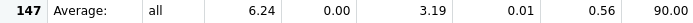
\includegraphics[width=\linewidth]{img/SC1_CPUAVG.png}
	\caption{Gemiddeld CPU gebruik (100 - Laatste Kolom).}
	\label{fig:SC1_CPUAVG}
\end{figure}
\begin{figure}[h]
	\centering
	\begin{minted}{bash} 
> summary(ram)
RAM       
Min.   :89.33  
1st Qu.:89.75  
Median :90.11  
Mean   :90.13  
3rd Qu.:90.39  
Max.   :91.25
	\end{minted}
	\caption{Gemiddeld RAM gebruik in Scenario 1}
	\label{SC1_RAMAVG}
\end{figure}

Ten tweede zullen de gegevens in verband met de stabiliteit van het systeem bekeken worden. In figuur \ref{fig:SC1_CPUBox} en \ref{fig:SC1_RAMBox} zijn de boxplots voor zowel het CPU als RAM gebruik te zien. We kunnen zien dat bij het CPU gebruik er maar drie \textit{outliers} zijn en bij het RAM gebruik zijn er zelf geen \textit{outliers}. Dit wijst erop dat het RAM gebruik zeer stabiel blijft. 

%\begin{figure}[ht]
%	\centering
%	\begin{minipage}[b]{0.75\linewidth}
%		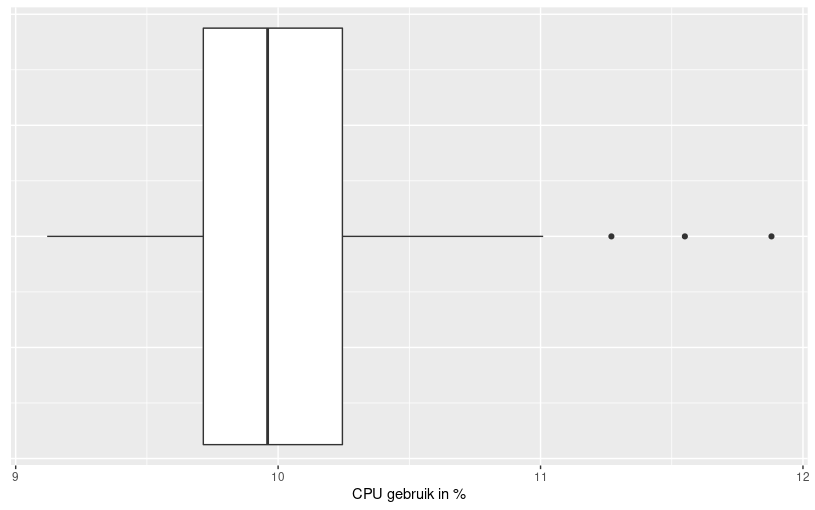
\includegraphics[width=\linewidth]{img/SC1_CPUBox.png}
%		\caption{Boxplot van het CPU gebruik in Scenario 1}
%		\label{fig:SC1_CPUBox}
%	\end{minipage}
%	\quad
%	\begin{minipage}[b]{0.75\linewidth}
%		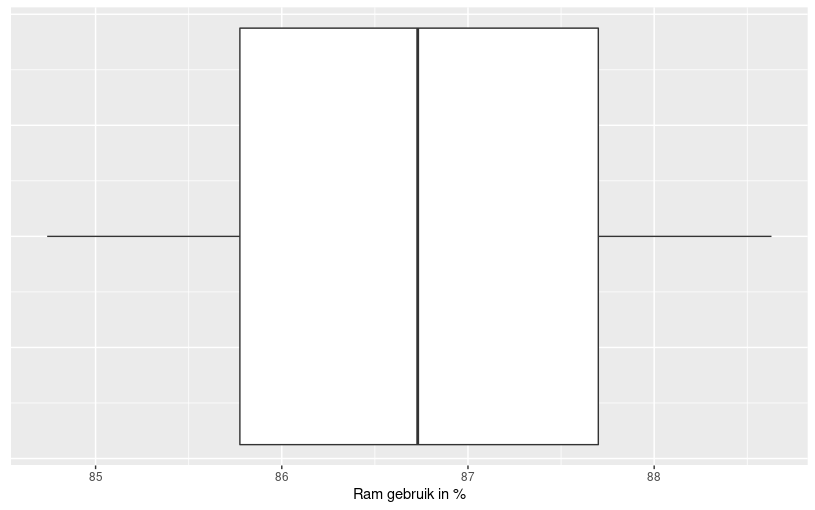
\includegraphics[width=\linewidth]{img/SC1_RAMBox.png}
%		\caption{Boxplot van het RAM gebruik in Scenario 1}
%		\label{fig:SC1_RAMBox}
%	\end{minipage}
%\end{figure}
%
\begin{figure}[h]
	\centering
	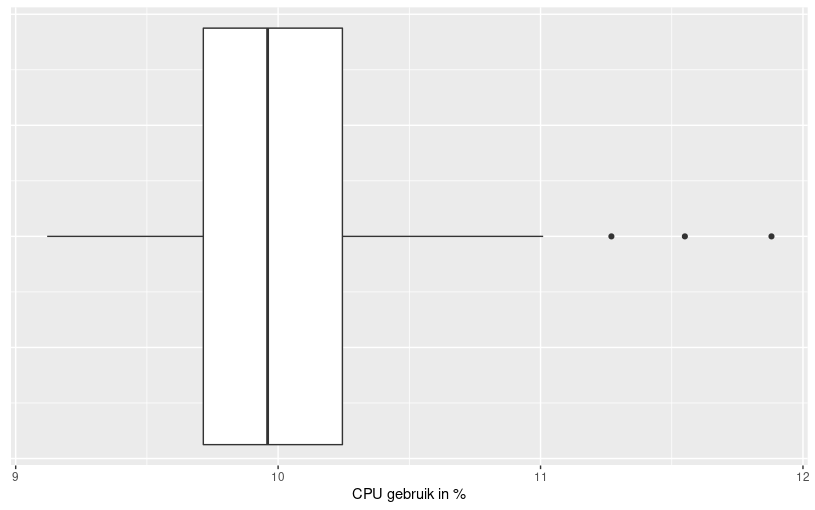
\includegraphics[width=0.75\linewidth]{img/SC1_CPUBox.png}
	\caption{Boxplot van het CPU gebruik in Scenario 1}
	\label{fig:SC1_CPUBox}
\end{figure}

\begin{figure}[h]
	\centering
	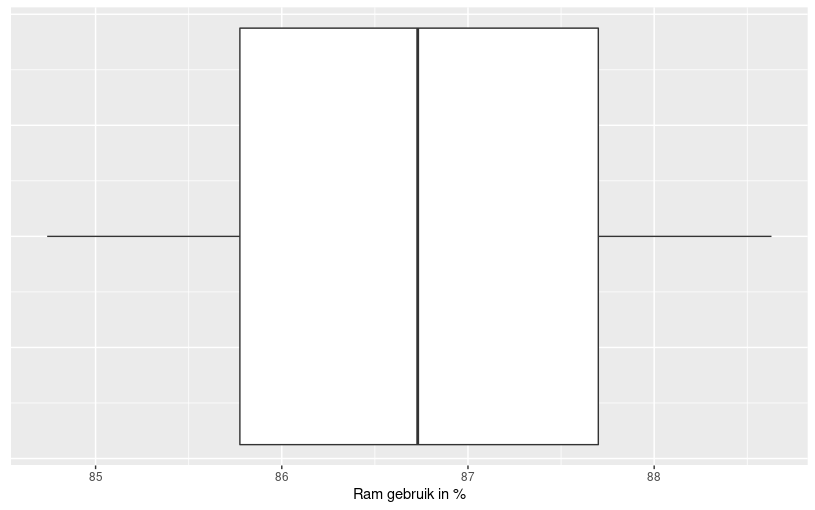
\includegraphics[width=0.75\linewidth]{img/SC1_RAMBox.png}
	\caption{Boxplot van het RAM gebruik in Scenario 1}
	\label{fig:SC1_RAMBox}
\end{figure}

Als derde criteria worden de gegevens van het algemene CPU en RAM gebruik bekeken. Deze worden gevisualiseerd aan de hand van een lijngrafiek. Het resultaat van scenario één is te zien in figuur \ref{fig:SC1_CPUGraph} en \ref{fig:SC1_RAMGraph}.

\begin{figure}[h]
	\centering
	\begin{minipage}[b]{0.45\linewidth}
			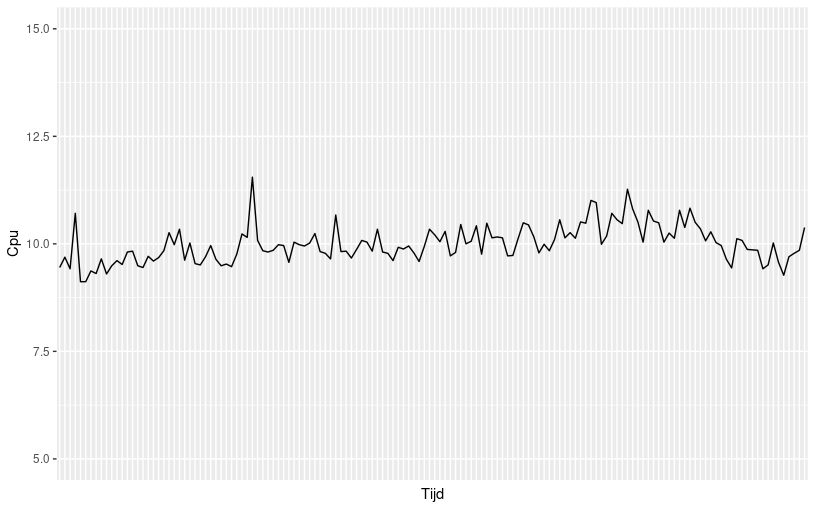
\includegraphics[width=\linewidth]{img/SC1_CPUGraph.png}
		\caption{Lijngrafiek van het CPU gebruik in Scenario 1.}
		\label{fig:SC1_CPUGraph}
	\end{minipage}
	\quad
	\begin{minipage}[b]{0.45\linewidth}
		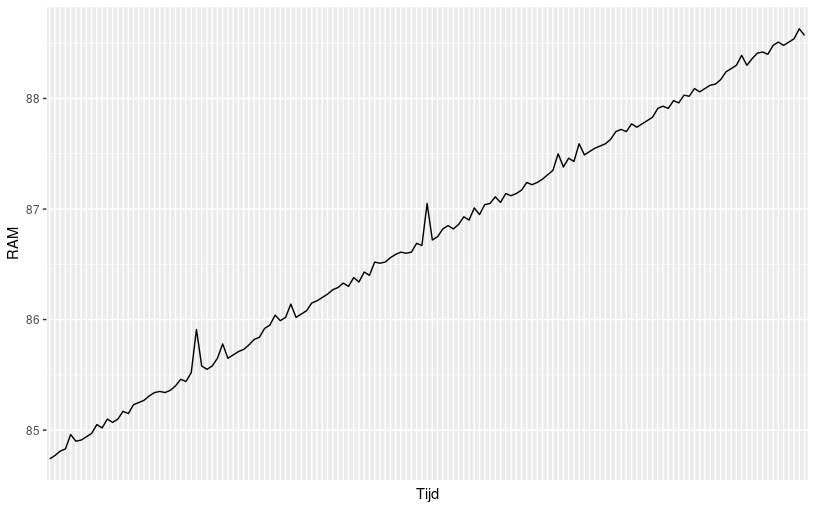
\includegraphics[width=\linewidth]{img/SC1_RAMGraph.png}
		\caption{Lijngrafiek van het RAM gebruik in Scenario 1.}
		\label{fig:SC1_RAMGraph}
	\end{minipage}
\end{figure}


Het laatste criteria is de opstarttijd van de node. Deze kan men simpelweg vinden aan de hand van het \verb|systemd-analyze| commando. De uitvoer van dit commando is te zien in figuur \ref{SC1_StartTime}.

\begin{figure}[h]
	\centering
	\begin{minted}{bash} 
$ systemd-analyze
Startup finished in 6.121s (kernel) + 3.296s (userspace) = 9.418s
	\end{minted}
	\caption{Opstarttijd van de Node in Scenario 1}
	\label{SC1_StartTime}
\end{figure}

%1e is gemiddelde
%2e is boxplot
%3e is Graph
%4e is opstarttijd

\clearpage
\subsection{Scenario 2}
% Node 45.79.249.208 wordt gebruikt
Als eerste zal het gemiddelde gebruik van zowel de CPU als het RAM geheugen verzameld worden. Voor de CPU is dit 10.15\% zoals te zien in figuur \ref{fig:SC2_CPUAVG}. Het gemiddelde RAM gebruik is af te lezen wanneer we de code uit figuur \ref{RAMAVG} uitvoeren op de dataset. De uitvoer hiervan is 90.75\%, zoals in figuur \ref{SC2_RAMAVG} te zien is.
\begin{figure}[h]
	\centering
	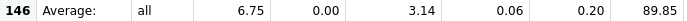
\includegraphics[width=\linewidth]{img/SC2_CPUAVG.png}
	\caption{Gemiddeld CPU gebruik (100 - Laatste Kolom).}
	\label{fig:SC2_CPUAVG}
\end{figure}
\begin{figure}[h]
	\centering
	\begin{minted}{bash} 
> summary(ram)
RAM       
Min.   :90.21  
1st Qu.:90.60  
Median :90.74  
Mean   :90.75  
3rd Qu.:90.91  
Max.   :91.27  
	\end{minted}
	\caption{Gemiddeld RAM gebruik in Scenario 2}
	\label{SC2_RAMAVG}
\end{figure}

Ten tweede zullen de gegevens in verband met de stabiliteit van het systeem bekeken worden. In figuur \ref{fig:SC2_CPUBox} en \ref{fig:SC2_RAMBox} zijn de boxplots voor zowel het CPU als RAM gebruik te zien. We kunnen zien dat bij het CPU gebruik er vier \textit{outliers} zijn en bij het RAM gebruik zijn er zelf geen \textit{outliers}. 

%\begin{figure}[ht]
%	\centering
%	\begin{minipage}[b]{0.75\linewidth}
%		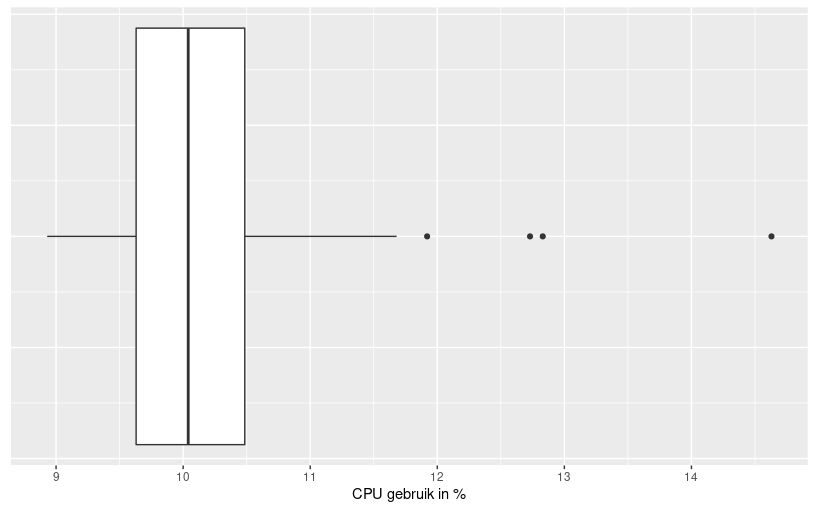
\includegraphics[width=\linewidth]{img/SC2_CPUBox.png}
%		\caption{Boxplot van het CPU gebruik in Scenario 2.}
%		\label{fig:SC2_CPUBox}
%	\end{minipage}
%	\quad
%	\begin{minipage}[b]{0.75\linewidth}
%		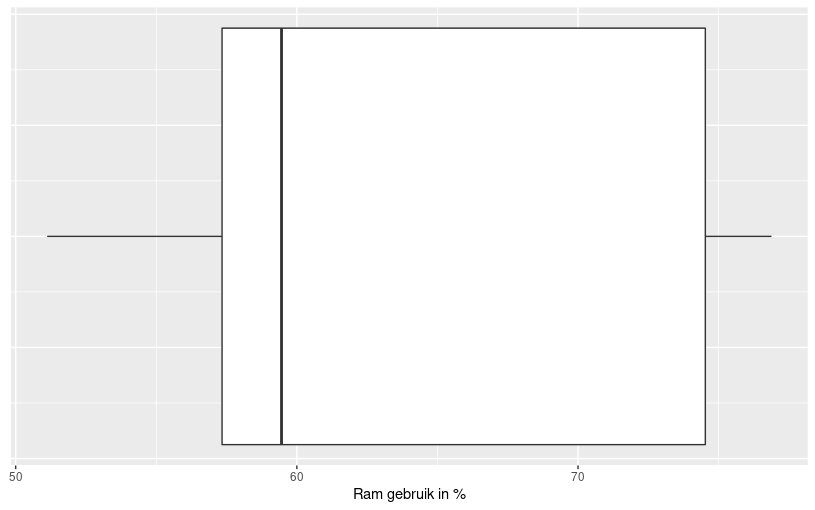
\includegraphics[width=\linewidth]{img/SC2_RAMBox.png}
%		\caption{Boxplot van het RAM gebruik in Scenario 2.}
%		\label{fig:SC2_RAMBox}
%	\end{minipage}
%\end{figure}
%
\begin{figure}[h]
	\centering
	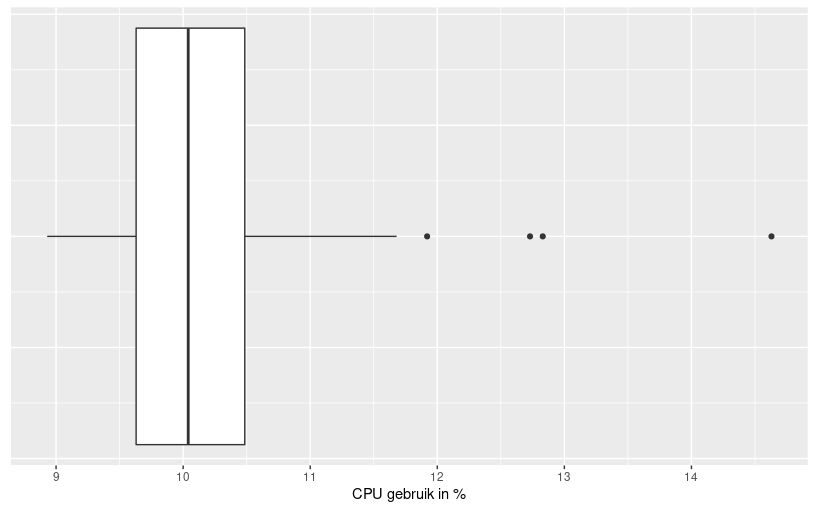
\includegraphics[width=0.75\linewidth]{img/SC2_CPUBox.png}
	\caption{Boxplot van het CPU gebruik in Scenario 2}
	\label{fig:SC2_CPUBox}
\end{figure}

\begin{figure}[h]
	\centering
	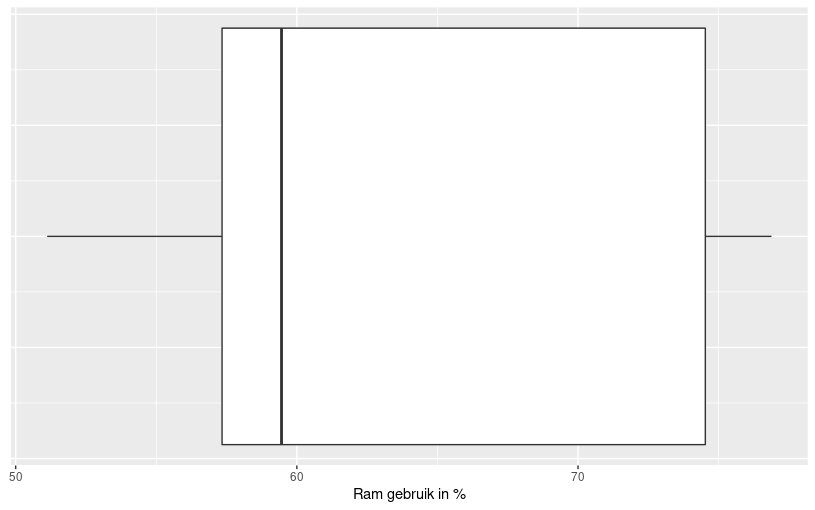
\includegraphics[width=0.75\linewidth]{img/SC2_RAMBox.png}
	\caption{Boxplot van het RAM gebruik in Scenario 2}
	\label{fig:SC2_RAMBox}
\end{figure}


Als derde criteria worden de gegevens van het algemene CPU en RAM gebruik bekeken. Deze worden gevisualiseerd aan de hand van een lijngrafiek. Het resultaat van scenario twee is te zien in figuur \ref{fig:SC2_CPUGraph} en \ref{fig:SC2_RAMGraph}. 
\begin{figure}[h]
	\centering
	\begin{minipage}[h]{0.45\linewidth}
		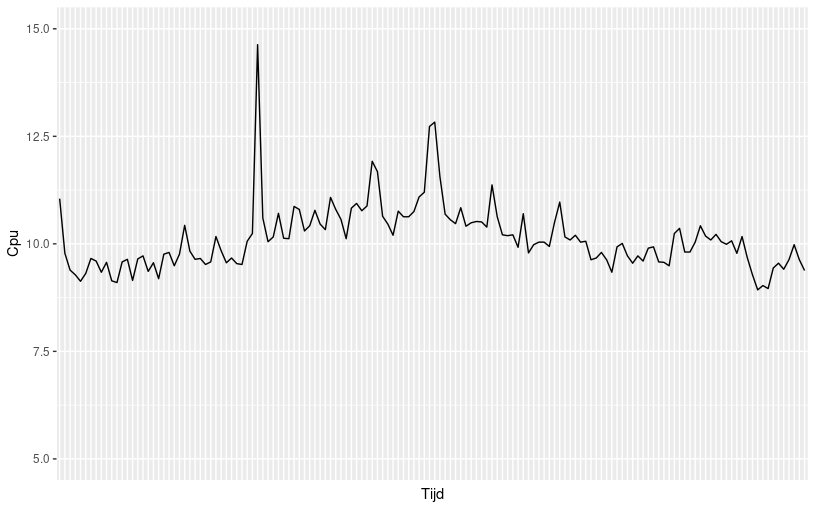
\includegraphics[width=\linewidth]{img/SC2_CPUGraph.png}
		\caption{Lijngrafiek van het CPU gebruik in Scenario 2.}
		\label{fig:SC2_CPUGraph}
	\end{minipage}
	\quad
	\begin{minipage}[h]{0.45\linewidth}
		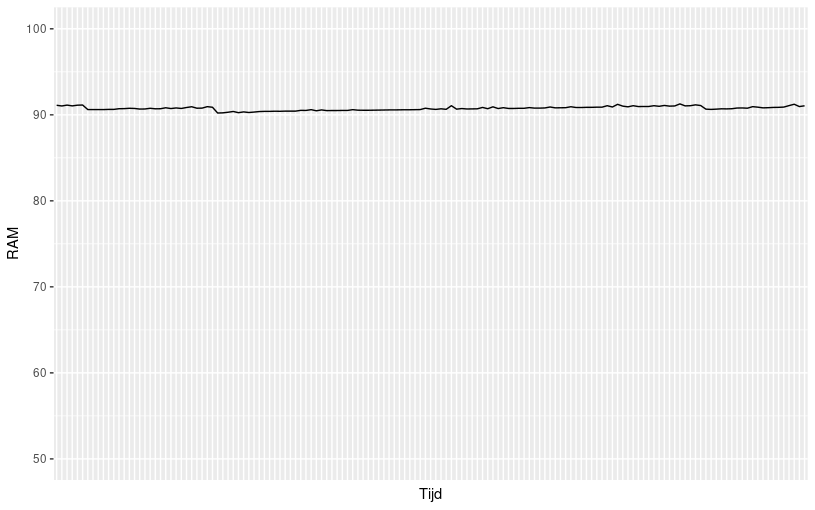
\includegraphics[width=\linewidth]{img/SC2_RAMGraph.png}
		\caption{Lijngrafiek van het RAM gebruik in Scenario 2.}
		\label{fig:SC2_RAMGraph}
	\end{minipage}
\end{figure}

%\begin{figure}[h]
%	\centering
%	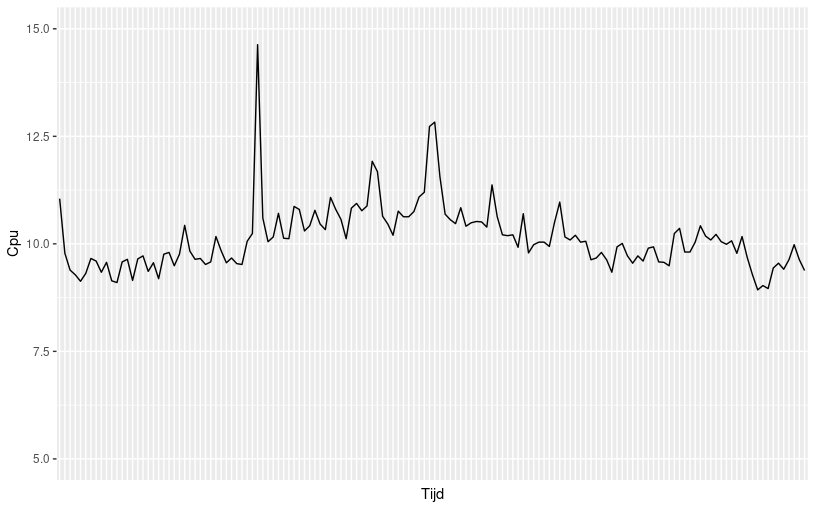
\includegraphics[width=0.75\linewidth]{img/SC2_CPUGraph.png}
%	\caption{Boxplot van het CPU gebruik in Scenario 2}
%	\label{fig:SC2_CPUGraph}
%\end{figure}
%
%\begin{figure}[h]
%	\centering
%	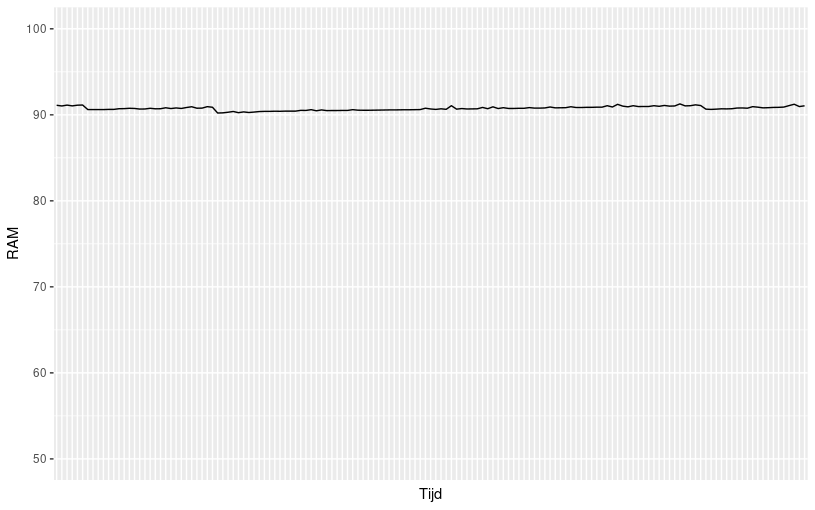
\includegraphics[width=0.75\linewidth]{img/SC2_RAMGraph.png}
%	\caption{Boxplot van het RAM gebruik in Scenario 2}
%	\label{fig:SC2_RAMGraph}
%\end{figure}


Het laatste criteria is de opstarttijd van de node. Deze kan men simpelweg vinden aan de hand van het \verb|systemd-analyze| commando. De uitvoer van dit commando is te zien in figuur \ref{SC2_StartTime}.

\begin{figure}[h]
	\centering
	\begin{minted}{bash} 
$ systemd-analyze
Startup finished in 6.246s (kernel) + 2.997s (userspace) = 9.243s
	\end{minted}
	\caption{Opstarttijd van de Node in Scenario 2}
	\label{SC2_StartTime}
\end{figure}

\clearpage
\subsection{Scenario 3}
% node 172.105.86.96 wordt gebruikt
%Data verzamelen over kube-bench door ./repeat.sh uit te voeren zodat dit zichtbaar is in de sar logs
%Kubebench even laten runnen zodat er een spike komt
%
%Kube hunter op de drie manieren uitvoeren op deze cluster 
%	op een node installeren
%	een node van de andere cluster scannen
%	een bad pod erin smijten

Als eerste zal het gemiddelde gebruik van zowel de CPU als het RAM geheugen verzameld worden. Voor de CPU is dit 12.3\% zoals te zien in figuur \ref{fig:SC3_CPUAVG}. Het gemiddelde RAM gebruik is af te lezen wanneer we de code uit figuur \ref{RAMAVG} uitvoeren op de dataset. De uitvoer hiervan is 90.13\%, zoals in figuur \ref{SC3_RAMAVG} te zien is.
\begin{figure}[h]
	\centering
	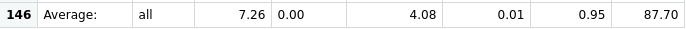
\includegraphics[width=\linewidth]{img/SC3_CPUAVG.png}
	\caption{Gemiddeld CPU gebruik (100 - Laatste Kolom).}
	\label{fig:SC3_CPUAVG}
\end{figure}
\begin{figure}[h]
	\centering
	\begin{minted}{bash} 
> summary(ram)
RAM       
Min.   :89.33  
1st Qu.:89.75  
Median :90.11  
Mean   :90.13  
3rd Qu.:90.39  
Max.   :91.25    
	\end{minted}
	\caption{Gemiddeld RAM gebruik in Scenario 3}
	\label{SC3_RAMAVG}
\end{figure}

Ten tweede zullen de gegevens in verband met de stabiliteit van het systeem bekeken worden. In figuur \ref{fig:SC3_CPUBox} en \ref{fig:SC3_RAMBox} zijn de boxplots voor zowel het CPU als RAM gebruik te zien. Bij het CPU gebruik zien we 11 outliers en bij het RAM gebruik zijn er geen outliers. Dit wijst er op dat het CPU gebruik minder stabiel blijkt te zijn in vergelijking met de vorige scenario's.

\begin{figure}[h]
	\centering
	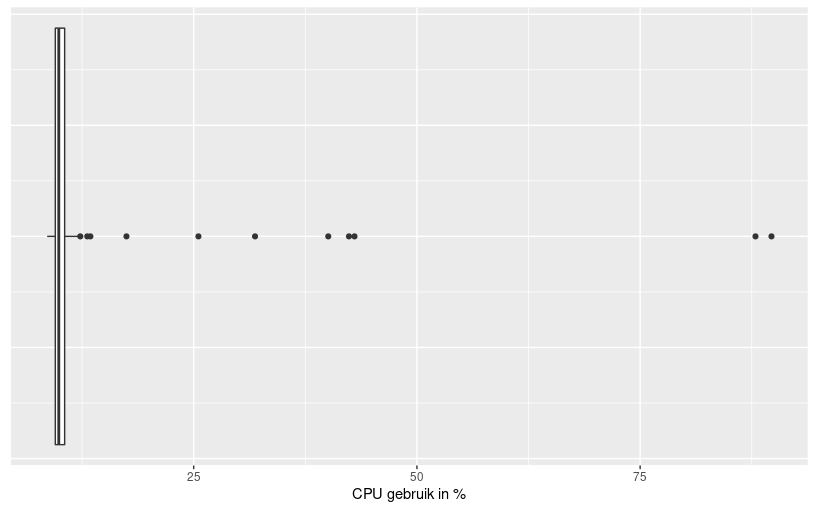
\includegraphics[width=0.75\linewidth]{img/SC3_CPUBox.png}
	\caption{Boxplot van het CPU gebruik in Scenario 3}
	\label{fig:SC3_CPUBox}
\end{figure}

\begin{figure}[h]
	\centering
	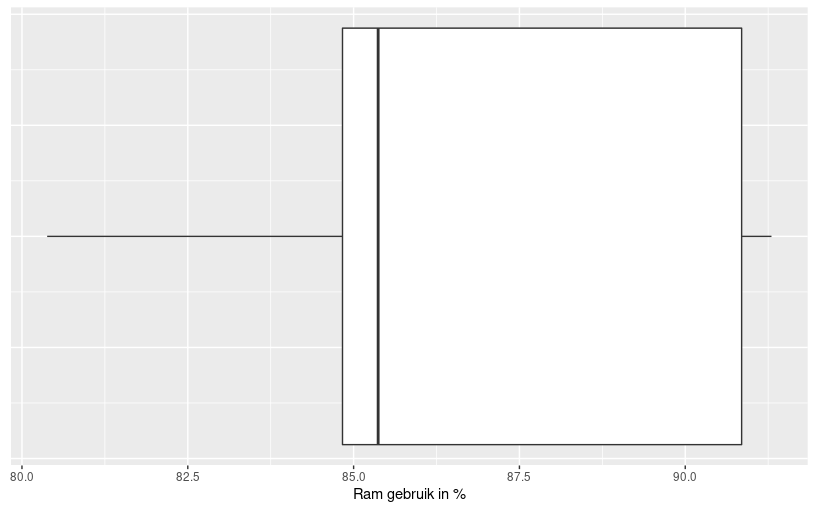
\includegraphics[width=0.75\linewidth]{img/SC3_RAMBox.png}
	\caption{Boxplot van het RAM gebruik in Scenario 3}
	\label{fig:SC3_RAMBox}
\end{figure}


Als derde criteria worden de gegevens van het algemene CPU en RAM gebruik bekeken. Deze worden gevisualiseerd aan de hand van een lijngrafiek. Het resultaat van scenario 3 is te zien in figuur \ref{fig:SC3_CPUGraph} en \ref{fig:SC3_RAMGraph}. De eerste piek in CPU gebruik is te wijten aan het gebruik van Kube-bench terwijl de tweede en derde piek zijn veroorzaakt door het gebruik van Kube-hunter.
\begin{figure}[h]
	\centering
	\begin{minipage}[h]{0.45\linewidth}
		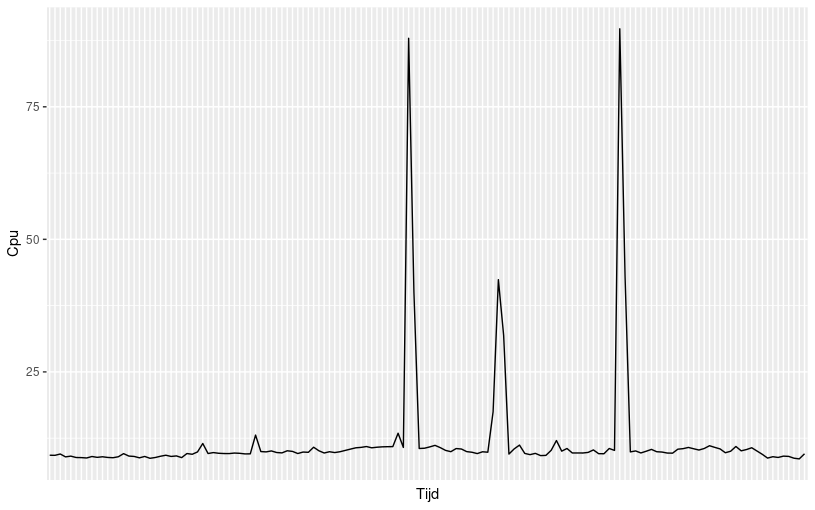
\includegraphics[width=\linewidth]{img/SC3_CPUGraph.png}
		\caption{Lijngrafiek van het CPU gebruik in Scenario 3.}
		\label{fig:SC3_CPUGraph}
	\end{minipage}
	\quad
	\begin{minipage}[h]{0.45\linewidth}
		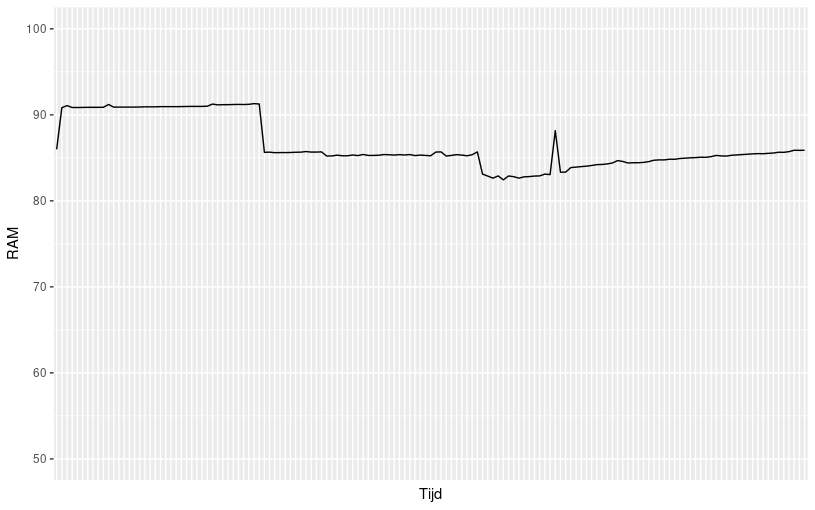
\includegraphics[width=\linewidth]{img/SC3_RAMGraph.png}
		\caption{Lijngrafiek van het RAM gebruik in Scenario 3.}
		\label{fig:SC3_RAMGraph}
	\end{minipage}
\end{figure}


Het laatste criteria is de opstarttijd van de node. Deze kan men simpelweg vinden aan de hand van het \verb|systemd-analyze| commando. De uitvoer van dit commando is te zien in figuur \ref{SC3_StartTime}.

\begin{figure}[h]
	\centering
	\begin{minted}{bash} 
$ systemd-analyze
Startup finished in 6.153s (kernel) + 5.180s (userspace) = 11.334s
	\end{minted}
	\caption{Opstarttijd van de Node in Scenario 3}
	\label{SC3_StartTime}
\end{figure}

\clearpage
\subsection{Vergelijken van de data}
Nu alle gegevens verzameld en verwerkt zijn kunnen we deze met elkaar gaan vergelijken. Als eerste zal het gemiddeld \textit{resource} gebruik van de verschillende scenario's besproken worden. Tabel \ref{tab:AVGResource} geeft een overzicht van de data. In deze tabel is duidelijk te zien dat zowel de \textit{best practices} als de beveiligings-tools een invloed hebben gehad op het CPU gebruik. De hoeveelheid RAM die gebruikt werd is daarentegen hetzelfde gebleven bij zowel scenario één als drie. Deze is in scenario twee zelfs gezakt. Ook al werden in scenario drie de tools maar sporadisch gebruikt, toch hebben deze een aanzienlijke impact op het gemiddeld \textit{resource} gebruik van de cluster gehad. 
\begin{table}[h]
	\centering
	\begin{tabular}{lccc}
		Gemiddeld resource gebruik & Scenario1 & Scenario2 & Scenario3 \\ \hline
		CPU                        & 10        & 10.15        & 12.3      \\ \hline
		Ram                        & 90.13     & 90.75        & 90.13    
	\end{tabular}
	\caption{Gemiddeld resource gebruik van de scenario's}
	\label{tab:AVGResource}
\end{table}

Het tweede criteria dat onderzocht werd is de stabiliteit van de cluster, dit door het aantal \textit{outliers} te tellen. In tabel \ref{tab:Outliers} is te zien hoeveel \textit{outliers} er per scenario werden gedetecteerd. Geen enkel scenario had effect op de stabiliteit van het RAM gebruik maar het CPU gebruik werd wel iets instabieler in scenario drie. Deze grote hoeveelheid \textit{outliers} is te wijten aan het feit dat de beveiligings-tools niet constant in gebruik zijn. De \textit{outliers} komen hier dus overeen met de momenten waarop de tools actief werden gebruikt. Hieruit is te concluderen dat \textit{best practices} een kleine (praktisch verwaarloosbare) impact hebben op de stabiliteit. Alsook dat beveiligings-tools een tijdelijke maar toch aanzienlijk effect hebben op de data.
%
\begin{table}[h]
	\centering
	\begin{tabular}{lccc}
		Aantal outliers & Scenario1 & Scenario2 & Scenario3 \\ \hline
		CPU             & 3         & 4         & 11        \\ \hline
		Ram             & 0         & 0         & 0        
	\end{tabular}
	\caption{Aantal outliers van de scenario's}
	\label{tab:Outliers}
\end{table}

Het laatste criteria dat werd onderzocht is de opstarttijd van een node in de cluster. Tabel \ref{tab:BootTime} toont de hoeveelheid seconden die de node in elk scenario nodig had om op te starten. Deze tabel maakt duidelijk dat \textit{best practices} geen (of in dit geval een positief) effect hebben op de opstarttijd van een cluster. De beveiligings-tools aan de andere kant zorgde er voor dat de nodes twee seconden trager opstarten. 

\begin{table}[h]
	\centering
	\begin{tabular}{lccc}
		& Scenario1 & Scenario2 & Scenario3 \\ \hline
		Opstarttijd & 9.418     & 9.243     & 11.334   
	\end{tabular}
	\caption{Tijd die de node nodig had om op te starten}
	\label{tab:BootTime}
\end{table}




% Voeg hier je eigen hoofdstukken toe die de ``corpus'' van je bachelorproef
% vormen. De structuur en titels hangen af van je eigen onderzoek. Je kan bv.
% elke fase in je onderzoek in een apart hoofdstuk bespreken.

%\input{...}
%\input{...}
%...

%%=============================================================================
%% Conclusie
%%=============================================================================

\chapter{Conclusie}
\label{ch:conclusie}

% TODO: Trek een duidelijke conclusie, in de vorm van een antwoord op de
% onderzoeksvra(a)g(en). Wat was jouw bijdrage aan het onderzoeksdomein en
% hoe biedt dit meerwaarde aan het vakgebied/doelgroep? 
% Reflecteer kritisch over het resultaat. In Engelse teksten wordt deze sectie
% ``Discussion'' genoemd. Had je deze uitkomst verwacht? Zijn er zaken die nog
% niet duidelijk zijn?
% Heeft het onderzoek geleid tot nieuwe vragen die uitnodigen tot verder 
%onderzoek?

\lipsum[76-80]



%%=============================================================================
%% Bijlagen
%%=============================================================================

\appendix
\renewcommand{\chaptername}{Appendix}

%%---------- Onderzoeksvoorstel -----------------------------------------------

\chapter{Onderzoeksvoorstel}

Het onderwerp van deze bachelorproef is gebaseerd op een onderzoeksvoorstel dat vooraf werd beoordeeld door de promotor. Dat voorstel is opgenomen in deze bijlage.

% Verwijzing naar het bestand met de inhoud van het onderzoeksvoorstel
%---------- Inleiding en State-of-the-art ---------------------------------------------------------

\section{Inleiding en State-of-the-art} % The \section*{} command stops section numbering
\label{sec:Inleiding en State-of-the-art}

\subsection{Wat zijn containers?}
Het uitrollen en schalen van applicaties wordt steeds vaker gedaan met behulp van containers. 
Tijdens de ontwikkeling van traditionele applicaties wordt de applicatie ontwikkeld in een specifiek testomgeving. 
Vervolgens wordt de applicatie overgezet naar de productieomgeving wat vaak voor problemen zorgt (bijvoorbeeld van een linux testomgeving naar een Windows productieomgeving). 
Een container is een pakket waar één enkele applicatie in zit, samen met alle nodige afhankelijkheden\autocite{Education2019}. 
Dit zorgt ervoor dat deze gemakkelijk en snel van de ene omgeving naar de andere kan overgezet worden. 
De containers maken gebruik van een 'runtime engine', dit is een laag die verantwoordelijk is voor de communicatie tussen het operating system van de host machine en de containers zelf. 
De meeste gebruikte 'runtime engine' is de 'Docker Engine'\footnote{https://docs.docker.com/engine/}. Deze is al sinds 2013 de industriestandaard als het gaat over container software\autocite{McCarty2018}. 
Naarmate het gebruik van containers steeg, steeg ook de nood naar op manier om deze vanuit één centrale locatie te beheren. 
Om aan deze vraag te voldoen werden container orkestratie tools, zoals Kubernetes \footnote{https://kubernetes.io/}, ontwikkeld. 
Deze tools helpen bij het opzetten, uitbreiden en verbinden van een grote hoeveelheid containers. 

\subsection{Waarom container applicaties?}
Container applicaties hebben enkele voordelen tegenover normale applicaties, ze draaien namelijk geïsoleerd van de rest van het systeem. 
Ze kunnen dus perfect werken zonder afhankelijk te zijn van andere containers. 
Dit garandeerd dat als er één container aangetast is, de rest zonder interruptie kan verderwerken. 
De containers delen wel verschillende resources van het host systeem, wat de deur opent voor veiligheidsinbreuken tussen containers. 

\subsection{Context voor dit onderzoek}
Gartner \autocite{Gartner2019} voorspeld dat tegen 2022 maar liefst 75\% van alle internationale organisaties gecontaineriseerde
applicaties zullen gebruiken in hun productieomgeving. Dit zowel in lokale datacenters alsook in online cloud omgevingen. 
Uit een raport van \textcite{Tripwire2019} blijkt dat 94\% van bevraagden bezorgd zijn over de veiligheid van hun containers. 
Uit hetzelfde raport blijkt ook dat 47\% weet dat ze kwetsbare containers gebruiken in hun productieomgeving. 
Spijtig genoeg werd bij voorgaande onderzoeken, zoals \textcite{StackRox2020}, het effect van 'security best practices en tools' 
op opzetsnelheid, benodigde resources en stabiliteit steeds onderbelicht. 

\subsection{Verloop van het onderzoek}
In deze paper zal ik onderzoeken wat de belangrijkste bronnen van veiligheidsinbreuken zijn en hoe deze vermeden kunnen worden. 
Tegelijkertijd krijg ik via dit onderzoek de opportuniteit om er achter te komen of er vooral technische problemen of menselijke fouten aan de basis liggen van de veiligheidsrisico's. 
In de volgende paragraaf staat er beschreven hoe ik te werk zal gaan. 

%---------- Methodologie ------------------------------------------------------
\section{Methodologie}
\label{sec:methodologie}

Voor dit onderzoek zullen er drie scenario's opgezet worden. Elk scenario zal verschillende keren worden uitgevoerd en voor elk criteria zal het genomen worden (eventueel reking houdende met uitschieters). 
Bij elke scenario zullen er verschillende 'security best practices en tools' gebruikt worden. 
Deze zullen getest worden op basis van de volgende criteria: \newline
\begin{itemize}
	\item Deployment snelheid
	\item Benodigde resources
	\item Stabiliteit \newline
\end{itemize} 
Voorbeelden van scenario's: \newline
\begin{itemize}
	\item S(0): Er wordt een container applicatie opgezet in een Kubernetes cluster zonder extra security configuratie.
	\item S(1): Er wordt een container applicatie opgezet in een Kubernetes cluster en enkele 'best practices' worden toegepast.
	\item S(2): Er wordt een container applicatie opgezet in een Kubernetes cluster waar er gebruik word gemaakt van enkele 'security tools' zoals 'Project Calico' en 'Kube-hunter'. \newline
\end{itemize} 
Door gebruik te maken van deze scenario's en criteria hopen we vast te stellen dat het toepassen van 'security best practices en tools' een positieve invloed heeft op het gebruik van containers en orkestratie tools. 

%---------- Verwachte resultaten ----------------------------------------------
\section{Verwachte resultaten}
\label{sec:verwachte_resultaten}

Op basis van de criteria wordt er verwacht dat Scenario 0 en 1 even snel op opgezet kunnen worden en evenveel resources gebruiken. 
Ze zullen beide kwetsbaarder zijn aangezien de 'best practices' vooral bestaan uit het correct gebruik van wachtwoorden en gebruiker privileges. 
Scenario 2 daarintegen zal iets meer tijd nodig hebben om opgezet te worden(zie Figuur1) en zal daarbij meer resources gebruiken(zie Figuur2). Dit zou te wijten zijn aan de gebruikte 'security tools' die extra tijd en resource nodig hebben. 

%---------- Verwachte conclusies ----------------------------------------------
\section{Verwachte conclusies}
\label{sec:verwachte_conclusies}

Uit dit onderzoek willen we concluderen dat het toepassen van 'best practices' en het correct gebruik van security tools een positief effect teweeg brengt bij het gebruik van container orkestratie tools. 
We trachten daarnaast ook aan te duiden dat het omzeilen van security risico's een belangrijk aspect is bij het ontwikkelen van container applicaties. 
Tot slot kan er geconcludeerd worden dat het beveiligen van container clusters steeds belangrijker wordt. 
Daarnaast is het tevens van belang dat de persoon die een cluster opzet daarbij de onderliggende werkwijze goed kent en zich bewust is van de mogelijke valkuilen. 

%---------- Bijlagen ----------------------------------------------
\section{Bijlagen}
\label{sec:Bijlagen}
\begin{figure}[ht]
	\centering
	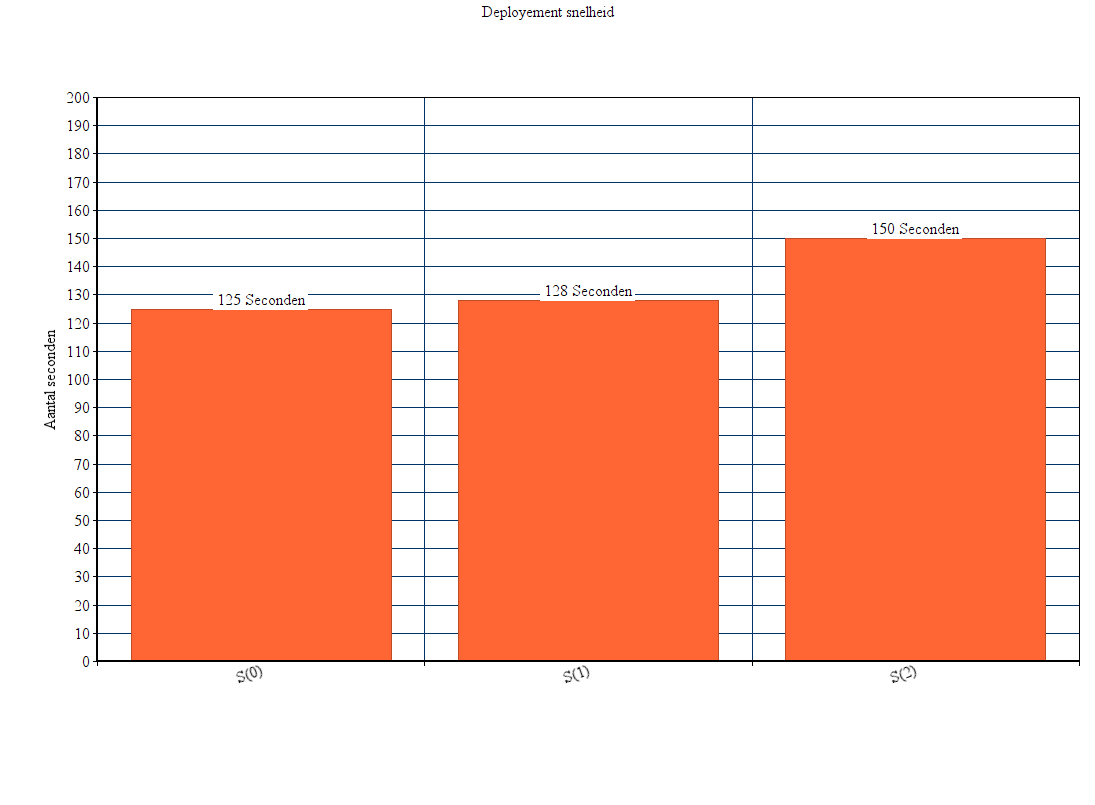
\includegraphics[width=\linewidth]{img/Mock1.png}
	\caption{Verwachte opstart tijd}
	\label{fig:example}
	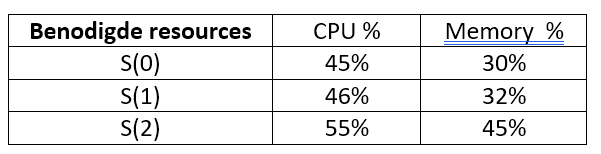
\includegraphics[width=\linewidth]{img/Mock2.png}
	\caption{Verwacht resource gebruik}
  \label{fig:example}
\end{figure}

%%---------- Andere bijlagen --------------------------------------------------
% TODO: Voeg hier eventuele andere bijlagen toe
%\input{...}

%%---------- Referentielijst --------------------------------------------------

\printbibliography[heading=bibintoc]

\end{document}
